{ \color{gray}
    %--- Move some of this to the introduction, perhaps, or to the chapter on fuzzy spheres. However, I think all what is related to an energy cutoff might be better placed here.
    
    
    % Why does it make sense to have an energy cutoff? At least $2$ reasons:
        
    %         \begin{enumerate}
                
    %         \item Where neither we nor the environment can bring a state to higher energies. This gives an effective description of the system which is, in principle, sufficient for determining all physical predictions \& is \textbf{simpler to work with}: \cite{FioreTheCase2020} ``yield a simpler low energy approximation $\cut {\mathcal T}$ of a well-defined quantum theory $\mathcal T$''
            
    %         \item We might add $\cut E$ as a point where higher energy physics is unknown. MINE: This means that the theory where no cutoff is introduced is not complete, and instead that we have to work with NC space to begin with to come up with a theory for energies above the cutoff.: \cite{FioreTheCase2020}``help in figuring out from the projected theory a new theory valid also at higher energies''
            
    %         \item \cite{FioreTheCase2020} Regularization procedure of a QFT theory: an energy cutoff $\cut E$ may allow to make sense of the theory if it is originally ill-defined due to UV divergences. More details in the intro of the paper: \cite{2020}``make sense of the original theory $\mathcal T$ if $\cut {\mathcal T}$ is well defined while $\mathcal T$ is not''
                
    %         \end{enumerate}
            
    % \cite{FioreTheCase2020}The following important observations may stem from the same energy cutoff procedure: introducing an energy cutoff $\cut E$ in a quantum theory on a commutative space(time) $M$, i.e. projecting the theory on the Hilbert subspace with energy below $\cut E$, directly induces a \rtext{noncommutative deformation of the latter [the Q. theory]} and \rtext{lower bounds for the space(time) locallyzability}. Moreover, adding a confining potential well $V$ with a very sharp minimum on a submanifold $N$ of $M$ may induce a dimensional \rtext{reduction to a noncommutative quantum theory on $N$} \rtext{\textbf{\Huge [Here the NC Quantum Theory is obtained from the energy cutoff, and that the resulting NC Theory is a NC approximation of Q. Theory on $N$ comes from the sharp potential; this last one is a \emph{dimensional reduction mechanism}!!}} ].
    %         \begin{enumerate}
            
    %         \item Regularization introducing energy cutoff was introduced for QED, although not Poincare covariant.
            
    %         \item DFR: concensus that any mergint of QM and GR should lead to a cutoff of local energy concentration (and an associated lower bound on localization of events). DFR made this more precise, and proposed that \rtext{the bound on the localizability of events could follow from appropriate NC coordinates}. (he cites a recent review: 10)
            
    %         \end{enumerate}
    
    % \lin 
    
    % \cite{FioreTheCase2020} First example of NC spacetime: Snyner in [6]: hope that \rtext{nontrivial commutation relations could cure ultraviolet divergences in QFT} But shortly after regularization introducing energy cutoff was introduced for QED, although not Poincare covariant.
    
%     \cite{FioreTheCase2020} Projecting a quantum theory onto the Hilbert subspace of states with energies below a cutoff $\cut E$ may\todo{why may? Do they simply refer to the possibility of this not being a general result?} \rtext{lead to an effective [quantum] theory with modified observables, including noncommutative space(time)}. 
    
%         \begin{itemize}
            
%         \item Let $S$ be a quantum system with algebra of observables $\acal = \bcal(\hcal)/Lin(\hcal)$ of bounded operators (with dense domain) over the Hilbert space $\hcal$ and hamiltonian $H$. e.g. \lbtext{low energy effective approximation} of the QM of a system: $\cut \hcal$ is spanned by eigenvectors of energies below a cutoff $\cut E$ e.g. (prototypical example) Peierls projection applied to the Landau model of a charged particle in a plane subject to a perpendicular magnetic field $B$; in that case, if $\cut E = E_0$ the ground state, then $[\cut x_1, \cut x_2] = \frac{i\hbar c}{ie B}$
        
%         \item Associated to any finite dimensional $\cut \hcal \subset \hcal$, let its \emph{algebra of observables} be defined as $\lbtext{\cut \acal} := End(\cut \hcal)$. Let $\cut P$ be the projection $\cut P : \hcal = \cut \hcal \oplus \cut H^\perp \to \cut \hcal$.
        
%         \begin{proposition}
%         \hfill
%         \begin{itemize}
            
%             \item Let $\cut{\acal}'$ be the subset of $\acal$ for which, if $\psi \notin \cut \hcal$, then $\cut \acal' \psi = 0$ and such that $Im(\cut \acal') \subset \cut \hcal$. Then $\acal'$ is a C$^*$-algebra isomorphic to $\cut \acal$ through the mappint $': \cut \acal \to \cut \acal'$ that extends an element on $\cut \acal$ to be $0$ in the orthogonal complement of $\acal'$.
            
%             \item Let $\overline{\quad}: \acal \to \cut \acal$, $A \mapsto \cut P A \cut P$. Then it is true that:
%             \begin{equation}
%                 (\cut A \cut B)' = \cut A' \cut B',
%             \end{equation}
%             for all $A, B \in \acal$.
            
%         \end{itemize}
%         \end{proposition}
%         \begin{notation}
%         This proposition allows us to think of $\cut \acal$ as $\cut \acal' \subset \acal$, and to operate elements $\cut A, \cut B \in \cut \acal$ that correspond to observables $A, B \in \acal$ using its corresponding elements in $\cut \acal' \subset \acal$. From now on we will ommit the $'$ notation and we will indistinctively let $\cut A$ be either an element of $\cut \acal$ and of $\cut \acal'$.
%         \end{notation}
         
        
%         For the low energy effective theories, given an observable $A$, e.g. $A = x_1$ in the Landau model, \rtext{$\cut A$ will % measure the SAME PHYSICAL QUANTITY with an uncertantiy compatible with $E \cut E$} here we find the corresponding commutation relations between ``position observables'']\todo{Although I'm not convinced that $\cut x$ is a good alternative version of $x$ in the projected theory, since it involves the action of $x$ itself which involves the creation of high energy eigenstates (), and THEN projecting... but I believe there might be a better notion of position measurement, although I do think that $\cut x$ might be an approximation. D'Andrea \cite{DAndrea2014} might have something to say about this.}
%         be a first approximation of the corresponding observable}
        
%         \item If $\cut \hcal$ is such that:
        
%             \begin{enumerate}[(i)]
            
%             \item $\cut P H = H \cut P$
            
%             \item $\cut A$ \todo{is this our case? This } contains all the observables corresponding to measurements that we can \emph{really} perform with the apparati at our disposal.
                
%             \end{enumerate}
            
%         Then, if the initial state belongs to $\hcal$ / the density matrix belongs to $\cut \acal$ then neither the dynamical evolution (generated by $H$) nor any measurement (due to (ii)) can map it out of $\cut \hcal$, and so \rtext{we can describe the effective theory of $S$ based on $\cut \hcal$, $\cut \acal$ and $\cut H = H|_{\cut \hcal}$}.
        
%         \item If $\hcal$ and $H$ (under the induced adjoint action on operators, equivalent to saying that this operator commuts with the group action) are invariant under some group $G$,then so are $\cut P$, $\cut \acal$ (within $\acal$), $\cut H$.
        
%         \rtext{Consequence}: if in the complete quantum theory of the system the coordinates $x_i$ commute (``commutative space''), this will not be in true, in general, for the effective theory: $[\cut x_i, \cut x_j] \neq 0$.
        
%         \end{itemize}
        
        
        
%     \cite{FioreTheCase2020} Adding a confining potential well $V$ with a very sharp minimum on a submanifold $N$ of the original space(time) $M$ may\todo{perhaps here the may refers to whether that is a correct interpretation of what is being done, since it might not be correct to say that we are doing $QM$ on $N$?} \rtext{induce a dimensional reduction to a \textbf{noncommutative quantum theory} on $N$} [the noncommutative quantum theory part, just as in the theory of Chakraborty and Scholtz, seems to mean that not only do the coordinates of phase space commute, but also that the space coordinates themselves do not commute.]
    
    
    
    
%     \lin   
    
%     $O(D)$-equivariance/covariance?
    
%         \begin{itemize}
            
%         \item \rtext{My best guess:} $O(2)$ acts by diffeomorphisms on the NC space.
            
%             \begin{itemize}
                
%             \item The action of $G$ makes things fall again in $\mathcal H_{\cut E}$, since it even makes an eigenvalue of $H$ fall again into an eigenvalue of $H$ with the same energy.
% $\Rightarrow$ $O(2)$ acts on $\mathcal H_{\cut E}$ $\Rightarrow$ $O(2)$ acts on $\mathcal A_{\cut E}$ by inner automorphisms, i.e. \rtext{$O(2)$ acts by diffeomorphisms on the NC space}.    
%             \item The time evolution of a ``rotated'' vector is simply given at any time as the rotation of the evolution of the orignal vector. Alternatively, $H^g = H$, so the time evolution of the a rotated vector is given by the same Hamiltonian.
            
%             \item The two above things imply that the evolution of a vector in $\mathcal H_{\cut E}$ is given by the same $H$, and that \rtext{this evolution is invariant under $O(2)$}
            
                
%             \end{itemize}
            
%         %\item Why make so much emphasis on ``the commutation relations (satisfied by the algebra generators) are $G$-invariant?'' And what does it even mean? {\tiny It can't be simply that $[A, B]^g = [A^g, B^g]$ since that is trivial to see given that $g$ acts by inner isomorphisms, and so it wouldn't be necessary to say that this is true since the commutation relations and $H$ (and hence) $P_{\cut E}$ are so... \rtext{but I think that's what makes sense since it would mean that the generated algebra is ``the same''}. It can't mean that $[A, B]^g = [A, B]$, since not even for the generators $\cut{x^\pm}$ that is true, since under reflections $\cut L$ does change.        }  
        
%         \item Fiore and Pisacane 2020: ``$O(D)$-covariance of the theory [$\mathcal T$ or $\cut{\mathcal T}$] means that for any orthogonal matrix $g \in O(D)$ there is a unitary transformation $U(g)$ of the [corresponding] Hilbert space $\hcal$ or $\cut \hcal$ such that $g^i_j v_j = U^\dagger(g) v_i U(g)$ for all vectors $\vec v$, and similary for other $O(D)$-tensors''. This, in the $D = 2$ case I have seen this to be satisfies for the $\vec{\cut x}$ observables, in which case it comes the commutation of the projection ($\rightarrow$ of $H$) with the $O(2)$-action.
        
%         \item For ``\lbtext{covariance}'': $G$ is a symmetry of the theory:
            
%             \begin{itemize}
                
%             \item $[g\cdot , H] = 0$ implies \otext{$[g\cdot , P_{\cut E}] = 0$}
            
%             \item That, in turn, implies that \otext{$\cut{A}^g = \cut{A^g}$}
                
%             \end{itemize}
            
%         \end{itemize}
    
    
%     \lin
    
%     Results \cite{FioreTheCase2020}:
%         \begin{itemize}
        
%         \item $\acal_\Lambda$ is a fuzzy approximation of the whole algebra of observables of the particle on $S^d$ (phase space algebra), and converges to the latter in the limit $\Lambda \to \infty$.
        
%         \item $\{\mathcal C_\Lambda\}$ can be interpreted as the space of functions on fuzzy configuration space $S^2_\Lambda$; while Madore's $\{\acal_\Lambda\}$ should be interpreted only as the space (actually, the algebra) of functions on a \emph{fuzzy spin phase space $S^2_n$}
            
%         \end{itemize}
    
}

Fiore and Pisacane in \cite{Fiore2018} and \cite{Fiore2019} build new fuzzy spheres from the introduction of an energy cut-off to quantum mechanics on euclidean spaces in which there is a near-harmonic potential around the unit sphere $r = 1$. More precisely, for a general dimension $D = d+1 \in \ZZ_{\geq 2}$, they first build a low energy effective theory for this system introducing an energy cutoff $\cut E \geq 0$. This includes the study of operators that that might play the role of representing certain observables in these effective theories like position. The resulting vector of position operators have the characteristic of transforming covariantly under the group $O(D)$ as expected from a position vector, but, interestingly, its coordinates no longer commute.

A sequence of such low effective theories can be made with increasingly higher energy cutoffs, and in the cases $D = 2$ and $D = 3$ they show that, in some precise sense, these theories have as ``commutative limit'' the quantum mechanics of a free spin-less particle in $S^d$. Under some additional restrictions on how the steepness of the harmonic potential increases between the terms of the sequence, Fiore and Pisacane show that these sequence are a fuzzy space that approximate the spheres $S^d$.

In this chapter we follow their construction for the case $D = 2$, including the presentation of some alternative algebras that are $*$-isomorphic in an $O(2)$-equivariant way to the original construction.

%%%%%%%%%%%%%%%%%%%%%%%%%%%%%%%%%%%%%%%%%%%%%%%%%%%%%%%%%%%%%%%%
%%%%%%%%%%%%%%%%%%%%%%%%%%%%%%%%%%%%%%%%%%%%%%%%%%%%%%%%%%%%%%%%
\section{Quantum Mechanics with near-harmonic Potential and an Energy Cutoff}
\label{chNewFuzzySectionGeneralSeting}

% {
%     \color{gray}
    
%     - $H = - \frac{1}{2} \Delta + V(r)$ invariant under $O(D)$
    
%     - Introducing the cutoff $\cut E$, as the energy where
%     \begin{align}
%         \label{eqn5}
%             V(r) \approx V_0 + 2k(r-1)^2 && \text{for $r$ such that $V(r) \leq  \cut E$}.
%     \end{align}
%     %in the region $\nu_{\cut E} = \{r \,|\, V(r) \leq \cut E\}$.
    
%     - Eigenfunctions of $H$ as product of a spherical harmonic $Y(\phi, \dots)$ (eigenvector of $L^2$) and an eigenfunction of the radial equation 
%     \begin{align}
%         \label{eqn9}
%         \left[-\partial_r^2 - (D-1) \frac{1}{r} \partial_r + \frac{1}{r^2} j(j+D-2) + V(r)\right] \tilde f(r) = E \tilde f(r).
%     \end{align}
%     - This last equation can be approximated by a harmonic oscillator equation, since outside the region $\{V(r) \leq \cut E\}$ $\psi$ is negligibly small.
%     : \rtext{$\hcal_{\cut E} \approx $ solutions of Schrodinger Eq. of energy $\leq \cut E$, $\acal_{\cut E} = End(\hcal_{\cut E})$}.
% }

\subsection{Algebras of Effective Observables $\mathcal{A}_{\cut E}$} 
%%%%%%%%%%%%%%%%%%%%%%%%%%%%%%%%%%%%%%%%%%%

In order to construct the new fuzzy spheres we need to develop a way to produce the individual algebras. These algebras will all be examples of the algebras $\acal_{\cut E}$ that we will now build.

In dimension $D = d + 1 \in \ZZ_{\geq 2}$, let $\hcal = L^2(\RR^D)$ be the Hilbert space of square integrable complex valued functions on $\RR^D$ (modulo identifications almost-everywhere). Suppose that the dynamics of a quantum spin-less particle described by the wavefunction $\psi(\vec r) \in \hcal$ is determined by the Schr\"odinger equation
\begin{equation} \label{SchrodingerEquationFullGeneralD}
    H \psi = i \frac{\partial}{\partial t} \psi,
\end{equation}
where the Hamiltonian operator $H$ of the system is of the form
\begin{equation}\label{equationHamiltonianGeneralD}
    H = -\frac{1}{2} \Delta + V(r);
\end{equation}
we are using natural units $\hbar = c = 1$, and assuming a unit mass $m = 1$. Here, $r$ is the radius in $\RR^D$, $V(r)$ is a radially symmetric potential and $\Delta = \sum_{i = 1}^D \frac{\partial}{\partial x^i} =: \sum_{i = 1}^D \partial_i \partial_i$ is the Laplacian on $\RR^D$, where $x^i$, $i = 1, \dots, D$ are the Cartesian coordinates on $\RR^D$. 

The first ingredient for the construction will be to let the potential be nearly harmonic with minimum value $V(1) = V_0$ at $r = 1$, i.e. such that
\begin{align}\label{equationPotentialHarmonicGeneralD}
            V(r) &\approx V_0 + 2k(r-1)^2 & k \geq 0
    \end{align}
in some region $\nu_{\tilde E} := \{r \,|\, V(r) \leq \tilde E\}$, for some value $\tilde E \geq V_0$. Actually, to obtain simple eigenvalues of the Hamiltonian, $V_0$ is  chosen such that the lowest energy $E$ is $0$, turning $V_0$ into a function of $k$. Moreover, we will suppose that $k = V''(r)/4 > 0$ is very large, so that $V(r)$ is a close to a confining potential for the particle into the $d$-sphere, $S^d$; this condition on $k$ will be made more precise below, when the cutoff energy is introduced.

\lin

The algebras that make a up the new fuzzy will be chosen as the space of observables of the vector subspace of $\hcal$ inside which no wavefunctions of energy higher that some cutoff energy inhabit. Hence, we need a description of the eigenfunctions of the energy operator, i.e. of the Hamiltonian. 
To do this, we use polar coordinates $r, \phi, \cdots$ where $r = \sqrt{\sum_i (x^i)^2}$ is the radius, and $\phi, \cdots$ are angles on $S^d$, so
\begin{equation}\label{LaplacianPolarCoordinatesGeneralD}
    \Delta = \partial_r^2 + (D-1)\frac{1}{r} \partial_r - \frac{1}{r^2} L^2,
\end{equation}
where, $p_i$, $i, j = 1, \dots, D$, is the linear momentum conjugate to $x^i$, and the operators $L_{ij} = i(x^i p_j - x^j p_i)$ are the angular momentum components, and so $L^2 = \frac{1}{2} \sum_{i, j} (L_{ij})^2$ is the square angular momentum operator, which is also the negative of the Laplacian on $S^d$ as the above equation shows if $r=1$. It is well known \cite{} that the eigenvectors of $L^2$, called the \dbtext{spherical harmonics}, have eigenvalues $j(j+D-2)$, for $j \in \ZZ_{\geq 0}$. 

For the eigenfunction $\psi$ of $H$ with eigenvalue $E$ we may use the ansatz
\begin{equation}\label{ansatzSolutionEigenfunctionEigenvalueEnergyHamiltonianGeneralD}
    \psi(r, \phi, \dots) = \tilde f(r) Y(\phi, \dots).
\end{equation}
Using separation of variables on the Schr\"odinger equation \eqref{SchrodingerEquationFullGeneralD} we deduce that \emph{$\psi$ is an eigenfunction of $L^2$ with eigenvalue $j(j+D-2)$}; this means that we may add a first label $j$ to the observable energy: $E_j$. On the other hand, the radial part of $\psi$ satisfies
\begin{align}\label{equationRadialSchrodingerGeneralDPolarAngles}
        \left[-\partial_r^2 - (D-1) \frac{1}{r} \partial_r + \frac{1}{r^2} j(j+D-2) + V(r)\right] \tilde f(r) = E_j \tilde f(r).
\end{align}

By Fuchs theorem \cite{}, for this equation to have a solution $V(r)$ needs to grow at most as $\beta/r^2$ when $r$ goes to $0$, for some $\beta \geq 0$, in which case equation \eqref{equationRadialSchrodingerGeneralDPolarAngles} has two independent solutions with asymptotic behavior $r^\alpha$ and $r^{-\alpha}$, respectively, as $r$ goes to $0$, where $\alpha = \sqrt{\beta + j(j+D-2)}$. For $\tilde f$ to be defined in the origin the contribution of the second solution must vanish, in particular $\tilde f(0) = 0$; for $\psi = \tilde f\, Y$ to be square integrable on $\RR^D$ it is required that $\tilde f(r) \to 0$ as $r$ goes to infinity.
We now see that the near confining harmonic potential \eqref{equationPotentialHarmonicGeneralD} implies that the energy eigenfunction $\psi$ becomes small outside the $\nu_{\cut E}$ region.
Finally, it can be shown \cite{Fiore2019} that the above equation can be approximated, for $r \approx 1$, by a harmonic oscillator equation
\begin{equation} \label{harmonicApproximationRadialSolutionGeneralD}
    [- \partial_{\tilde r} + \tilde k_j(\tilde r - \tilde r_{j})^2] f(\tilde r) = \tilde E_j \tilde f(r)
\end{equation} 
for some $\tilde r$ function of $r$, $f(\tilde r) := \tilde f(r)$ and $\tilde k, \tilde r_j$ constants and, furthermore, that \emph{the lowest eigenvalue solutions of the Schr\"odinger equation are approximately the solutions of the above harmonic oscillator equation}. Then, at least for the lowest eigenvalue solutions $\psi = \tilde f(r) Y(\phi, \dots)$ of the Schr\"odinger equation, the respective energies will have two labels: a label $j \in \ZZ$ coming from the angular factor $Y(\phi, \dots)$, and a label $n \in \ZZ_{\geq 0}$ coming from the radial part $\tilde f(r)$: $E_{n, j}$.

\lin

\begin{figure}[h][h]
    \centering
    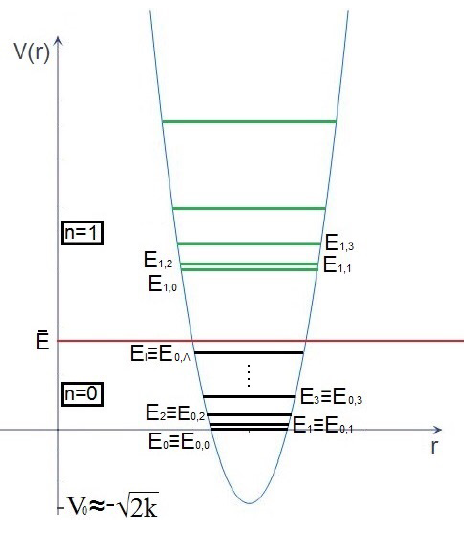
\includegraphics[width = 2\textwidth/3/2]{images/FioreEigenvalues.PNG}
    \caption{Eigenvalues of the Hamiltonian for steep enough potential for $D = 2$. The cutoff energy $\cut E$ can be chosen so that the energies below it are the spectrum of the free Hamiltonian $L^2$ in $S^d$. Image extracted from \cite{Fiore2018}}
    \label{fig:D2EigenvaluesEigenEnergiesHarmonicCutoff}
\end{figure}

As illustrated in \ref{fig:D2EigenvaluesEigenEnergiesHarmonicCutoff}, if $k$ is steep enough% small enough with respect to $k$, e.g. $\cut E \lesssim 8\sqrt{k}$, 
the eigenvalues of $H$ below $E_{1,0}$ will be a truncation of the spectrum of $L^2$, i.e. the smallest eigenvalues of $H$ will be (approximately) $j(j+D-1)$ for $j = 0, 1, 2, \dots, \Lambda$ for some $\Lambda \in \NN$. This introduces the second main ingredient of our construction: \emph{the energy cutoff}. In general:
\begin{definition}\label{definitionAcalHcalGeneralD}
Let the dimension $D = d + 1 \in \ZZ_{\geq 2}$ be arbitrary. Given an energy $\cut E \geq 0$, suppose that $k$ is sufficiently steep to make the eigenvalue $E_{1, 0}$ be above $\cut E$, now called the cutoff energy. %\dbtext{but also that $\cut E$ is high enough so that no eigenvalues are between it and $E_{1, 0}$} 
Then, we will define the algebra \lbtext{$\acal_{\cut E}$} as the algebra of operators over the finite dimensional Hilbert space \lbtext{$\hcal_{\cut E}$}, spanned by the solutions $\psi_{0, j} \equiv \psi_j$ of the Schrodinger equation (under the harmonic oscillator approximation \eqref{harmonicApproximationRadialSolutionGeneralD}) whose energies $E_j := E_{0, j}E_j$ are below $\cut E$.
\end{definition}

\lin 

Finally, in order to make a fuzzy space $\{\acal_\Lambda\}_{\Lambda \in \NN}$ out of this construction of algebras $\acal_{\cut E}$, we need to make $\cut E$ and $k$ grow with a $\Lambda \in \NN$ in such a way that:
\begin{enumerate}
    \item $k$ is big enough to not produce radial excitations, i.e. keep nontrivial radial eigenfunctions, rhose for which the label $n \geq 1$, above the cutoff;
    
    \item for fixed $\Lambda$, the maximum proper energy is $\Lambda(\Lambda + D - 2)$. This may be done by choosing 
\begin{align}
    \cut E = \cut E(\Lambda) &= \Lambda(\Lambda + d - 1), & k = k(\Lambda) \geq \Lambda^2(\Lambda + 1)^2.
\end{align}
\end{enumerate} 

\lin 

We now make a series of observations about the constructed algebras:

\begin{remark}
Since the Hamiltonian operator is the generator of time evolution for a quantum system, a \rtext{ quantum system that is setup in a state $\psi \in \hcal_{\cut E}$ will not evolve out of $\hcal_{\cut E} \subset \hcal$}. More precisely, recall that the eigenvectors of the Hamiltonian operator are called \dbtext{steady-state states} since their time evolutions consists only of a change of phase, leaving invariant the probability distribution they induce and, in particular, staying as states of constant energy. 
%since the Hamiltonian is hermitian, it is diagonalizable and every wavefunction can be written \todo{Always? In the f.d. case this is true} as a (countable)\todo{Como es que se llama esto? La alternative a Hamel basis} linear combination of eigenfunctions of $H$; 
Hence, if $\psi_0 \in \hcal_{\cut E}$, it is a linear combination of eigenfunctions of $H$ of energy lower than $\cut E$ and, by applying the linear time-evolution operator $\exp[-itH] = 1 - itH - t^2 H^2 + \cdots$, $\psi(t) := U(t) \psi_0$ will once again be a linear combination of eigenfunctions of $H$ with low energy, i.e. $\psi(t)$ is also in $\hcal_{\cut E}$.
\end{remark}

\begin{remark}\label{remarkODActsOnHCutE}
The orthogonal group $O(D)$ is defined as the subset of the matrices $M_D(\RR)$ acting on the vectors of $\RR^D$ that respects the inner product of $\RR^d$, i.e. for any $\vec v, \vec w \in \RR^D$, every matrix $A \in O(D)$ satisfies $(A \vec v) \cdot (A \vec w) = \vec v \cdot \vec w$; it is easily shown that this condition is equivalent to $A^t A = 1_D$, where the subscript $\cdot ^t$ denotes the transpose matrix. This group contains not only all possible rotations on $\RR^D$, the group $SO(D) = \{A \,:\, det(A) = 1, \, A \in O(D)\}$, but also the reflections with respect to every hyperplane on $\RR^D$. 

\noindent $O(D) \ni g$ acts naturally from the left on $\RR^D$, and so it also acts on functions $\psi$ of $\RR^D$, in particular on $\hcal = L^2(\RR^D)$, through the unitary representation $\pi$ defined by $\pi(g)\psi: \vec v \to \psi(g^{-1} \vec v)$. Actually, \rtext{$O(D)$ acts on $\hcal_{\cut E} \subset \hcal$, and, therefore, on $\acal_{\cut E}$ from the left by inner automorphisms}, meaning that the action of any $g \in O(D)$ on any function $\psi \in \hcal_{\cut E}$ produces again a function in $\hcal_{\cut E}$. This follows from the fact that the Hamiltonian \eqref{equationHamiltonianGeneralD}, being radially symmetric, is $O(D)$-invariant, and so $[H, \pi(g)] = 0 \in \bcal(\hcal)$ for the action of any $g \in O(D)$, which implies that, if $\psi_E$ is an eigenfunction of $H$ of energy $E \leq \cut E$, then $\pi(g) \psi_E$ is also an eigenfunction for the same energy.%; then, acting on any $\psi \in \hcal_{\cut E}$, being a linear combination of such eigenfunctions, $g\cdot \psi$ is also in $\hcal_{\cut E}$.
Theorem \ref{theoremGeneralDEffectiveLowEnergyQuantumIsODCovariant} describes an additional property of the action of $\acal_{\cut E}$ under $O(2)$ when position observables are introduced.
\end{remark}

\subsection{Low Energy Effective Quantum Theories and their Properties}
%%%%%%%%%%%%%%%%%%%%%%%%%%%%%%%%%%%%%%%%%%%

\subsubsection{Projected Observables}

For every cutoff $\cut E$, and $k$ compatible with it, the Hilbert space $\hcal_{\cut E}$ together with the time evolution operator $H|_{\cut E}$ may be called a \emph{low energy effective quantum theory} of the quantum mechanics of the particle on $\RR^D$ subject to a potential that is nearly harmonic near $r = 1$, associated to the algebra of observables $\acal_{\cut E}$. To make the interpretation of the (hermitian) elements of $\acal_{\cut E}$ as the space that represents the observables and to justify calling it a quantum theory, based on Fiore and Pisacane \cite{Fiore2018} we \todo{they do not say this explicitly, but that seems to be what they asssume}\todo{or perhaps do not talk directly about measurement, but of the projection valued measures?} say that a measurement of an observable $B \in \acal_{\cut E}$ on the state $\psi \in \hcal_{\cut E}$ means to apply $B$ to $\psi$ and then return as the measured quantity an eigenvalue of $B$ with probability given by the norm of the projection of $B \psi$ in the corresponding eigenspace of $B$. 
Furthermore, at least for $D = 2$ we see in proposition \ref{theoremConvergesToQMD2} that a sequence of such low energy approximations with increasing $\cut E$, as that given by a fuzzy space, converge to the quantum theory of a spin-less particle in $S^1$.

Fiore and Pisacane in \cite{Fiore2018} propose a way to define an element $\cut A \in \acal_{\cut E}$ for each $A \in \bcal(\hcal)$ which, in case that $A$ represents an observable (i.e. $A$ is hermitian) then $\cut A$ may\todo{Again, this may is because what ``the theory'' really is we are not told, and also considering that they introduce AND work with other operators, namely $\chi$ here, as if they were the position observables } be considered the representation of the same observable in the low energy effective quantum theory:
\begin{proposition}\label{propositionCutACutObservableDefinitionMultiplication}
        \hfill
        \begin{itemize}
            
            \item Let $\acal_{\cut E}' \subset \acal$ be the subalgebra that annihilates $\hcal_{\cut E}^\perp$ and such that $\acal_{\cut E}' \hcal_{\cut E} \subset \hcal_{\cut E}$. Then $\acal_{\cut E}'$ is a C$^*$-algebra isomorphic to $\acal_{\cut E}$ through the mapping $': \cut \acal \to \cut \acal'$ defined, for each $B \in \acal_{\cut E}$, by $B'|_{\hcal_{\cut E}} = B$ and $B'|_{\hcal_{\cut E}^\perp} = 0$.
            
            \item For any densely defined operator $A$ on $\hcal$ whose domain includes $\hcal_{\cut E}$ (or whose action can be continuously extended to all of $\hcal_{\cut E}$), define $\cut A = P_{\cut E} A P_{\cut E} \in \acal_{\cut E}'$. Then:
            \begin{equation}
                (\cut A \cut B)' = \cut A'\, \cut B',
            \end{equation}
            for all $A, B$ operators for which the $\cut{{\color{white}L}}$ map can be applied.
        \begin{proof}
        This is a straightforward application of the definitions.
        \end{proof}
        \end{itemize}
        \end{proposition}
        \begin{notation}\label{notationCutOverline}
        This proposition allows us to think of $\cut \acal$ as a subalgebra $\cut \acal'$ of $\acal$, and to operate elements $\cut A, \cut B \in \cut \acal$ that correspond to observables $A, B \in \acal$ using its corresponding elements in $\cut \acal' \subset \acal$. From now on we will omit the $'$ notation and we will indistinctively let $\cut A$ be either an element of $\cut \acal$ of of $\cut \acal'$. given $A \in \bcal(\hcal)$.
        \end{notation}
         
        
        %For the low energy effective theories, given an observable $A$, e.g. $A = x_1$ in the Landau model, \rtext{$\cut A$ will % measure the SAME PHYSICAL QUANTITY with an uncertantiy compatible with $E \cut E$} here we find the corresponding commutation relations between ``position observables'']\todo{Although I'm not convinced that $\cut x$ is a good alternative version of $x$ in the projected theory, since it involves the action of $x$ itself which involves the creation of high energy eigenstates (), and THEN projecting... but I believe there might be a better notion of position measurement, although I do think that $\cut x$ might be an approximation. D'Andrea \cite{DAndrea2014} might have something to say about this.}
        %be a first approximation of the corresponding observable}

In particular, $\cut{x^i} \in \acal_{\cut E}$, $i, j = 1, \dots, D$ are candidates for the position observables within the effective quantum theory and, although $[x^i, x^j] = 0$, the additional projection operator implies that, in general: 
\begin{equation}
    [\cut x^i, \cut x^j] \neq 0.
\end{equation}
Other candidates for position operators will also be used, and the criteria of Section \ref{subsectionCriteriaGOodApproximationsOfPosition} is used to decide whether some operators are acceptable as candidates position operators in a sequence of algebras that approximate a quantum theory.

\subsubsection{$O(D)$-Covariance}

Let $(\mathcal H, \mathcal A, H)$ be a ``quantum theory'', like quantum mechanics on $\RR^D$: $(\hcal = L^2(\RR^D), \bcal(\hcal), H)$ where $H$ is any %radially symmetric 
Hamiltonian%\eqref{equationHamiltonianGeneralD}
, or quantum mechanics on $S^d$: $(L^2(S^d), \bcal(\hcal), H)$ for some Hamiltonian $H$, or any low energy effective theory: $(\hcal_{\cut E}, \acal_{\cut E}, \cut H)$ as defined in \ref{definitionAcalHcalGeneralD}. In all of these theories, whenever a group $G$ acts on $\hcal$, $G$ also acts on $\acal$ by inner automorphisms. In some cases this transformation satisfies certain properties, in which case we will call it a $G$-covariant theory according to Fiore and Pisacane \cite{FioreTheCase2020}:

\begin{definition}\label{definitionGActsCovariantlyOnCoordinates}
Let $\{\cut \hcal, \cut \acal = End(\cut \hcal), \cut H\}$ be a quantum theory as described above, and let $G$ be a subgroup of $M_D(\RR)$, for some $D \in \ZZ_{\geq 1}$ that acts on $\hcal$ through a unitary representation $\cut \pi: G \to \cut \acal$.
    \begin{itemize}
        
        \item Suppose that there are operators $x^i$ on $\hcal$, $i = 1, \dots, D$, where each $x^i$ is considered the representation of the observable of $i$-th coordinate of position. We say that \emph{the position coordinates transform contravariantly under $G$}, where $G$ is a subgroup of $M_D(\RR)$ if $G$ acts on $\hcal$ through a unitary representation and if 
        \begin{equation}
            \cut \pi(g) x^i \cut \pi(g)^* = \sum_{j = 1}^D (g^{-1})^i_j x^j.
        \end{equation}\todo{In 2020 they define a theory to be covariant if something like this applies to any ``vector'' and ``tensor'', but I'm not sure what they mean}
        
        \item Suppose that there are elements $p_i$ operators on $\hcal$, $i = 1, \dots, D$, where each $p_i$ is considered the representation of the observable of $i$-th coordinate of momentum. We say that \emph{the momentum coordinates transform covariantly under $G$}, where $G$ is a subgroup of $M_D(\RR)$ if $G$ acts on $\hcal$ through a unitary representation  and if 
        \begin{equation}
            \cut \pi(g) p_j \cut \pi(g)^* = \sum_{j = 1}^D g^i_j p_i.
        \end{equation}
    
    \item When the previous two conditions are satisfied, we say that \emph{the theory is $G$-covariant}.
    
    \end{itemize}
    \end{definition}

We now see some important examples of covariant theories, including the low energy effective quantum theories developed in this chapter.

\begin{proposition}\label{propositionQMIsODCovariantGeneralD}
For any $D \in \ZZ_{\geq 1}$, quantum mechanics on $\RR^D$ is an $O(D)$-covariant theory.
\end{proposition}
\begin{proof}
For this statement to make sense, we first see that $O(D) \subset M_D(\RR)$ acts on the left on $\RR^D$ by multiplication, and so it acts on $\psi \in L^2(\RR^D)$ by $\pi(g)\psi(\vec x) := \psi(g^{-1}\vec x)$. To see that this representation of $O(D)$ on $\hcal = L^2(\RR^D)$ is unitary it suffices to see that
\begin{equation*}
    \langle \pi(g) \psi_1 | \pi(g) \psi_2\rangle =\int_{\RR^D} \overline{\psi_1}(g^{-1}\vec x) \psi(g^{-1}\vec x) d\vec x = \int_{\RR^D} \overline{\psi_1}(\vec x) \psi(\vec x) d\vec x = \langle \psi | \psi\rangle,
\end{equation*} 
for all $g \in O(D)$ and $\psi_1, \psi_2 \in L^2(\RR^D)$; we used that the measure of $\RR^D$ is invariant under $O(D)$. 

Now we can go on to prove that the position and momentum coordinates transform covariantly. Let $g \in G$, $\psi \in \hcal$ and $i \in \{1, \dots, D\}$ be arbitrary, then:
\begin{align*}
    \pi(g)^* x^i \pi(g) \psi(\vec x) 
    &= \pi(g)^* x^i \psi(g^{-1} \vec x)\\
    &= \pi(g)^* f(\vec x) \\
    &= \pi(g^{-1}) f(\vec x)\\
    &= f(g\vec x) \\
    &= (g\vec x)^i \psi(g g^{-1} \vec x)\\
    &= \left( \sum_{j = 1}^D g^i_j x^j \right) \psi(\vec x),
\end{align*}
where $f(\vec x) = x^i \psi(g^{-1} \vec x)$, since $g$ and $\psi$ are arbitrary, we have thus proved that the the position coordinates operators transform contravariantly. 
Now, invert the relation $(g \vec x)^i = \sum_j g^i_j x^j$ in $\RR^D$ to conclude that $x^j = \sum_{i} (g^{-1})^j_i (g \vec x)^i$ for all $j \in \{1, \dots, D\}$. This implies that 
\begin{align*}
    \pi(g^{-1}) p_{i} \pi(g) \psi(\vec x) &= \pi(g^{-1})(-i \partial_{x^i}) \psi(g^{-1}\vec x) = -i \partial_{(g \vec x)^i} \psi(\vec x), &\text{for all }\psi \in L^2(\RR^D)\\
     \text{but }\quad \partial_{(g \vec x)^i} &= \sum_j \partial_{(g \vec x)^i} x^j \,\partial_{x^j}
     = \sum_j (g^{-1})^j_i \partial_{x^j},
\end{align*}
proving that the momentum operators transform $O(D)$-covariantly.
\end{proof}

From the previous proposition, the following important property of the low energy effective quantum theories developed in this chapter follows:
\begin{theorem}\label{theoremGeneralDEffectiveLowEnergyQuantumIsODCovariant}
For any $\cut E \in \RR^+$, let $\hcal_{\cut E}$ and $\acal_{\cut E}$ define a low effective quantum theory according to Definition \ref{definitionAcalHcalGeneralD}. Then, using $\cut {x^i}$ as position coordinate operators and $\cut {p_i}$ as momentum operators, this theory is $O(D)$-covariant
\end{theorem}
\begin{proof}
This fact is a combination of proposition \ref{propositionQMIsODCovariantGeneralD} with the invariance of the Hamiltonian $H$ \eqref{equationHamiltonianGeneralD} under $O(D)$ that follows from its radial symmetry, i.e. $\pi(g)^* (-\frac{1}{2} \Delta + V(r)) \pi(g) = -\frac{1}{2} \Delta + V(r)$ for all $g \in O(D)$, where $\pi$ is the unitary representation of $O(D)$ on $\hcal = L^2(\RR^D)$. The invariance of $H$ can be rewritten as $[H, \pi(g)] = 0$ by composing the previous relation with $\pi(g)$ to the left. The last relation implies that if $\psi$ is such that $H \psi = E \psi$ for some $E \in \RR$, then $H(\pi(g)\psi) = E(\psi(g)\psi)$, meaning that acting with $O(D)$ keeps an eigenvector in its corresponding eigenspace, and so, in particular, that $[P_{\cut E}, \pi(g)] = 0$.

Recall the notation \ref{notationCutOverline}. It follows that for any operator $A$ on $\hcal$ such that $\cut A = P_{\cut E} A P_{\cut E} \in \acal_{\cut E}$ is well defined and:
\begin{align*}
    \pi(g^*) \cut A \pi(g) 
      &= \pi(g)P_{\cut E} A P_{\cut E} \pi(g)\\
      &= P_{\cut E} \pi(g^*) A \pi(g) P_{\cut E}\\
      &= \cut{\pi(g^*) A \pi(g)}.
\end{align*}
Thus, the combination of the last equality with proposition \ref{propositionQMIsODCovariantGeneralD}, and the linearity of the $\cut{\color{white} A}$ map prove the theorem.
\end{proof}


\begin{proposition}\label{propositionMadoreISSO3Covariant}
Suppose that each element $\acal_N = \pi_{N/2}(U(\sut))$ of the fuzzy sphere \ref{definitionFuzzySphere} is considered a quantum theory over the irreducible spin $j = N/2$ representation space $V_{j}$. Take the algebra generators $\hat x^i = \frac{1}{\sqrt{j(j+1)}}\pi_j(J^i)$, defined in \ref{equationDefinitionGeneratorsFuzzySphere} for $i = 1, 2, 3$, as the representations of the $i$-th coordinate of the position observable. Then, for even $N$ the position coordinates transform $SO(3)$-contravariantly.
\end{proposition}
\begin{proof}
If $N$ is even, the irreducible representation on $V_j$ of the simply connected Lie group $SU(2)$, also denoted by $\pi_j$, quotients to an irreducible representation $\hat \pi_N$ of $SO(3)$. This follows from the fact that $SU(2)$ is its double cover, where the covering map $c:SU(2) \to SO(3)$ sends each element and its negative to the same $SO(3)$ element, combined with the fact that $\pi_j$ sends $-1 \in SU(2)$ to $1 \in End(V_j)$ for integer $j$.

That $SU(2)$ is the double cover of $SO(3)$ implies that there is an $(SU(2), SO(3))$-equivariant isomorphism $\sut \cong \soth$, hence $U(\sut) \cong U(\soth)$, where the isomorphism is such that $J^i \mapsto \hat J^i$, where $J^i$ are the generators of $U(\sut)$ with the commutation relations \eqref{equationCommutationRelationJs} and where $i \hat J^i$ is the infinitesimal rotation with respect to the $i$-th axis in $\RR^3$, i.e. $e^{i\theta J^i}$ is the rotation of an angle $\theta$ with respect to the $i$-th axis. Every rotation $R(\hat n, \theta)SO(3)$ is determined by an axis of rotation $\hat n$ and an angle of rotation $\theta$, and it is equal to 
\begin{equation*}
    R(\hat n, \theta) = \exp[i \theta \vec {\hat J}\cdot \hat n ],
\end{equation*} where $\vec{\hat J} = (\hat J^1, \hat J^2, \hat J^3)$. It can be shown that, given any other rotation $g \in SO(3)$
\begin{equation}\label{equationAdjointActionOnRotations3DBecomesRotationOfAxis}
    g R(\hat n, \theta) g^{-1} = R(g^{-1} \hat n, \theta),
\end{equation}
and since, by properties of the adjoint map, $g\exp[i \theta \vec {\hat J}\cdot \hat n ] g^{-1} = \exp[i g\theta \vec {\hat J}\cdot \hat n g^{-1}] = \exp[i \theta (g\vec {\hat J}g^{-1})\cdot \hat n ]$, where $g \vec {\hat J}g^{-1}$ is notation for $\sum_k g \hat J^k g^{-1}$, the previous equation implies, by differentiating the above equation with respect to $\theta$ at $0$ we conclude that
\begin{equation}\label{equationAdjointActionsOnHatJsGeneratorsofRotationsInfinitesimal}
    (g \vec{\hat J} g^{-1})\cdot \hat n = (g^{-1} \hat n) \cdot \vec{\hat J}.
\end{equation}
In particular, replacing for $\hat n$ equal to $(1, 0, 0)^T$, $(0,1,0)^T$ or $(0,0,1)^T$ this equation becomes
\begin{eqnsplit}\label{equationContravariantTransformationOfHatJsGeneratorsofSO3}
    g\hat J^k g^{-1} = \sum_i (g^{-1})^k_i \hat J^i.
\end{eqnsplit}
respectively, for $k = 1$, $k=2$, $k=3$. The representation $\hat \pi_N$ of the group $SO(3)$ is equivalent to an algebra representation $\hat \pi_N$ of $U(\soth)$, so applying it on both sides results in
\begin{equation}\label{equationContravariantTransformationOfJsSO3}
    \hat \pi_N(g) \pi_j(J^k) \hat \pi_N(g)^* = \sum_i (g^{-1})^k_i \pi_j(J^i),
\end{equation}
where we used the $(SU(2), SO(3))$-equivariance of the isomorphism $U(\sut)$ $\cong U(\soth)$ to conclude that $\pi_j(J^k) = \hat \pi_N(\hat J^k)$.

Thus, the $SO(3)$-contravariance transformation of the operators $\hat x^i = \frac{1}{\sqrt{j(j+1)}}\pi_j(J^i)$ follows.
\end{proof}

Under a simple multiplication of the definition of $G$-contravariance transformation of the coordinates, the previous proposition can be generalized to the statement that, for each $N \in \NN$, the position coordinates $\hat x^i$ defined in \eqref{equationDefinitionGeneratorsFuzzySphere} transform contravariently under $SU(2)$.

\lin

\subsubsection{Criteria for Position Observables}\label{subsectionCriteriaGOodApproximationsOfPosition}

% In the case of the position observables an exact measurement necessarily involves the use of high energy probes, producing a ``position eigenfunction'' the wavefunction collapses would be a delta distribution which includes a contribution from all energy eigenfunctions; hence, $\cut x^i = P_{\cut E} x^i P_{\cut E}$ which involves the measurement of $x^i$, followed by a projection, may not be a good operator that represents the measurement $x_i$ in the effective theory.
Suppose that there is a sequence of quantum theories, with algebras $\{\acal_N\}_{N \in \NN}$, whose limit is the quantum theory of a spin-less particle on $S^d$; theorem \ref{theoremConvergesToQMD2} proves that this is the case for the low energy effective theories associated to a fuzzy space produced through the constructions of this chapter. Fiore and Pisacane in \cite{FioreXi2020} propose the following minimal criteria for a set of operators $\chi^i \in \acal_N$, $i = 1, \dots, D$, with spectrum $\Sigma^N_i$, $N \in \NN$, to be a good $O(D)$-covariant approximation of the position operators $x^i$ on $L^2(S^d)$:
    \begin{enumerate}
    
    \item For all $N$, the spectrum $\Sigma^N_i$ of $\chi^i$ is invariant under the action of $O(D)$, including inversion $x^i \mapsto -x^i$. In particular, the spectra $\Sigma_i$ of $\chi^i$ are all equal.
    
    \item The sequence of spectra $\{\Sigma_i^N\}_{N \in \NN}$ becomes uniformly dense\footnote{For any point $x \in [-1, 1]$ and any open ball $U \subset [-1, 1]$ containing $x$, there is some $N \in \NN$ such that, for all $n \geq N$, $U \cup \Sigma_i$ is not empty, and, furthermore, it is evenly distributed within $U$} in $[-1, 1]$ in the limit $N \to \infty$. In particular, the maximal and minimal eigenvalues are a sequence converging to $-1$ and $1$, respectively.
    
    \end{enumerate}

    
\begin{proposition}\label{propositionMadoreCoordinatesAreSO3ContravariantCovariant}
On the elements of the fuzzy sphere $\acal_N$ indexed by even $N$, let $\hat x^i = \frac{1}{\sqrt{j(j+1)}}\pi_j(J_i) \in \acal_{2j} = End(V_j)$, $2j \in \NN$. Then these operators satisfy the criteria, but replacing the group $O(3)$ by $SO(3)$.
\end{proposition}
\begin{proof}
 We saw in proposition \ref{propositionMadoreISSO3Covariant} that those algebra elements transform $SO(3)$-contravariently; we will bring the notation from the proof of said proposition. %This was basically derived from the fact that $\hat x ^i = \frac{1}{\sqrt{j(j+1)}} \hat \pi_N(\hat J^i)$, where $iJ^i$ is the infinitesimal rotation with respect to the $i$-th axis. In general, an infinitesimal rotation on $\RR^3$ has the form $\vec{\hat J} \cdot \hat n$ for some $\hat n \in \RR^3$ unitary that indicates the axis of rotation. 
 Equation \eqref{equationAdjointActionsOnHatJsGeneratorsofRotationsInfinitesimal} means that acting with $g \in SO(3)$ on the infinitesimal rotation $i \vec J \cdot \hat n$ produces again an infinitesimal rotation, namely $i (g^{-1} \hat n)\cdot \vec J$, and so the spectrum of $\hat \pi_N(J^i)$ is invariant under actions of $SO(3)$. Thus, the spectrum of each $\hat x_i$ given $N$ is
 \begin{equation*}
     \Sigma^N_i = \left\{-\sqrt{\frac{j}{j+1}}, \frac{-j+1}{\sqrt{j(j+1)}}, \dots, \frac{j-1}{\sqrt{j(j+1)}},  \sqrt{\frac{j}{j+1}}\right\},
 \end{equation*} is invariant under the action of $SO(3)$. 
 
 The sequence of spectra is clearly uniformly dense in $[-1, 1]$.
 
 %and the group $O(3)$ acts naturally on $U(\sut) \cong U(\soth)$, and hence on $A_{2j} = \pi_j(U(\sut))$, and this action coincides with the expected action of $O(D) \ni g$ on coordinate functions: $g\, (x^1, \dots, x^D)^T = (g\cdot x^1 , \dots, g \cdot x^D)^T$, where $g \cdot x^i = \frac{1}{\sqrt{j(j+1)}}\pi_j(g J_i g^{-1})$. Similarly, we will see in \ref{} that this criteria will be satisfied for the new Fuzzy sphere with $d = 2$ if the operators chosen as position coordinates are $\chi^i = \frac{\sqrt{2}}{a} \cut x^i$ as defined in $\ref{}$.
\end{proof}


%%%%%%%%%%%%%%%%%%%%%%%%%%%%%%%%%%%%%%%%%%%%%%%%%%%%%%%%%%%%%%%%
%%%%%%%%%%%%%%%%%%%%%%%%%%%%%%%%%%%%%%%%%%%%%%%%%%%%%%%%%%%%%%%%
\section{Construction of $\acal_{\cut E}$ for $D = 2$}

% {
%     \color{gray}
    
%     - Equation \eqref{eqn9} has the approximation, where $\rho := \ln r$
%     \begin{equation}
%         \label{harmonic2D}
%         \hat H f(\rho) = e_m f(\rho), \qquad
%         \hat H = - \partial_\rho^2 + k_m(\rho - \tilde \rho_m)^2,
%     \end{equation} $
%         k_m := 2(k - E'), \quad
%         E' := E - V_0, \quad
%         \tilde \rho_m := \frac{E'}{k_m}, \quad
%         e_m = \frac{E'^2}{k_m} + E' - m^2
%     $
%     - The solutions $f_{n,m}$ are known, $n \in \bb N, m \in \ZZ$ \then $e_{m, n}(k) = (2n+1)\sqrt{k_m}$ \then $E'_{m,n}(k)$ satisfies a quartic equation \then $E_{m,n}(k, V_0)$.
    
%     - Fixing $V_0 = V_0(k)$ such that $E_{0, 0} = 0$ \then $V_0(k) = -\sqrt{2k} + 2 - \frac{7}{2}\frac{1}{\sqrt{2k}} + o(1/k)$ and 
%     $\sum_{n = -1}^\infty v_n \left( \sqrt{\frac{1}{k}} \right)^n \approx -\sqrt{2k} + 2 - o(1/k)$ \then
%     \begin{equation}
%         \rtext{E_{n, m}(k)} = m^2 + 2n\sqrt{2k} - 2n + o(1/\sqrt{k})
%     \end{equation}
    
%     - Choosing $\cut E < 2 \sqrt{2k} - 2$, the spectrum of $H$ is a truncation of $L^2$: \textbf{the radial oscillations are ``frozen''}: $\cut{\partial_r} = 0$.
%     \begin{multline*}
%         \lbtext{\psi_m(\rho, \phi)} := f_{0, m}(\rho) e^{im\phi} = c_m e^{im\phi}exp{\left[ -\frac{(\rho - \tilde \rho_m)^2 \sqrt{k_m}}{2} \right]} \\\xrightarrow{k \to \infty} \delta(r-1)e^{i m \phi}
%     \end{multline*}
%     \begin{equation}
%         E = E_m(k) = m^2 + o(1/\sqrt{k})
%     \end{equation}
    
%     - For $\lbtext{\Lambda} := \lfloor \cut E \rfloor$, 
%     \begin{align}
%         \lbtext{\hcal_{\Lambda}}:= \lbtext{\hcal_{\cut E}} := span\{\psi_m\}_{|m| \leq 
%     \lfloor \cut E \rfloor} ,
%     \lbtext{\acal_\Lambda} := \mathcal B(\hcal_\Lambda)
%     \end{align}
    
%     - Since $H$ generates the time evolution, a
%     An element of $\hcal_\Lambda$ doesn't evolve out of $\hcal_\Lambda$.
    
%     - Get a fuzzy space: e.g. choosing $k = \Lambda^2(\Lambda+1)^2$ --make $k$ diverge with $\Lambda$ while $\nu_{\cut E}$ goes to $\{r = 1\}$
    
%     - This cutoff entails replacing every observable by $A \mapsto \lbtext{\cut A} = P_{\cut E} A P_{\cut E}$% \dbtext{when?}
% }


When decomposing the eigenfunctions of the Schrodinger equation into radial and angular components, $\psi(r, \phi) = \tilde f(r) Y(\phi)$, the angular equation $L^2 Y = EY$ for $D = d+1 = 2$ is 
\begin{equation}
    - \partial_\phi^2 Y = E Y
\end{equation}
since the only angular momentum component is $L_{12} = - L_{21} =:-i(x^1 \partial_2  - x_2 \partial_1) = - i \partial_\phi$, we define the angular momentum operator to be
\begin{equation}\label{equationAngularMomentumD2d1PartialPhi}
    L:= -i \partial_\phi    
\end{equation}
The \dbtext{spherical harmonics} are, then, labeled by an integer $m$ and:
\begin{align}
    Y_m(\phi) &= e^{im \phi} & m \in \ZZ\\
    E_m &= m^2.
\end{align}

\lin

Defining $\rho := \ln r$ and $f(\rho) := \tilde f(r)$, the radial equation \eqref{equationRadialSchrodingerGeneralDPolarAngles} becomes $f''(\rho) + \{e^{2\rho} [E - V(e^\rho)] - m^2 \} f(\rho) = 0$, and expanding $e^{2\rho}$ about $\rho = 0$ we obtain the following harmonic approximation of the radial equation \eqref{equationRadialSchrodingerGeneralDPolarAngles}\todo{Up to what order in $\rho$ or $r$ do these solutions coincide with the radial part of the action Schrodinger solution?}: 
\begin{equation}\label{equationHarmonicApproximation2DRadial}
        [- \partial_\rho^2 + k_m(\rho - \tilde \rho_m)^2] f(\rho) = e_m f(\rho),\text{ where}
\end{equation}
\begin{equation}\label{equationConstantsHarmonicApproximationRadialD2}
        k_m := 2(k - E'_m),\quad 
        E'_m := E_m - V_0,\quad 
        \tilde \rho_m := \frac{E'_m}{k_m},\quad
        e_m = \frac{E'^2_m}{k_m} + E'_m - m^2.
\end{equation} 
When solving this equation, taking into account that $\psi = f(\rho)Y(\phi) $ an additional label $n \in \ZZ_{\geq 0}$ appears for the eigenvalues of the previous equation; these solutions are:
\begin{eqnsplit}
    f_{n, m}(\rho) &= N_m \exp\left[ - \frac{(\rho - \tilde \rho_m \sqrt{k_m})}{2}\right] H_n\left[ (\rho - \rho_m)\right]\\
    e_{n, m} &= (2n+1) \sqrt{k_m},
\end{eqnsplit}
where $N_m$ is a normalization constant and the $H_n$ are the Hermite polynomials, $H_n$ being a polynomial of degree $n$ on the dependent variable; in particular, $H_0 = 1$.

From equation \eqref{equationConstantsHarmonicApproximationRadialD2} it follows that $E'_m \equiv E'_{n, m} = E_{n, m} - V_0$ satisfies
\begin{equation}\label{equationAlmostQuarticDeterminesE'}
    \frac{E'_{n, m}}{2(k - E'_{n, m})} + E'_{n, m} - m^2 = (2n+1) \sqrt{2(k - E'_{n, m})};
\end{equation}
by squaring both sides we obtain a quartic equation for $E'_{n,m}$ that makes it a function of $k$, and hence we obtain the original eigenvalues of the approximate Schr\"odinger equation $E_{n,m}$ as a functions of $k$ and $V_0$.

\lin

As was mentioned in the previous section, in order to get simple eigenenergies we fix $V_0$ such that the ground energy $E_{0, 0}$ equals $0$. To do this we replace $m = n = 0$ in equation \eqref{equationAlmostQuarticDeterminesE'} and use $E_{0, 0} = 0$. From there, we deduce that $V_0$ has a quartic equation that determines it a function of $k$ that can be rewritten as:
\begin{equation}\label{equationV0AlternativeNotQuartic}
    - \sqrt{\frac{1}{2k}}V_0 - \left( \sqrt{\frac{1}{2k}} \right)^3 V_0^2 = \left( 1 + \frac{V_0}{k} \right)^\frac{3}{2}.
\end{equation}
$V_0(k)$ has a unique solution root over the reals, although it is possible to find a closed formula for it since it is determined by a quadratic equation, we opt for the use of its Taylor series expansion with respect to the variable $1/\sqrt{k}$, at $k = \infty$, by using the implicit formula \eqref{equationV0AlternativeNotQuartic}; the resulting expansion is:
\begin{equation}\label{equationFormulaExpansionV0functionOfK}
    V_0(k) = - \sqrt{2k} + 2 - \frac{7}{2} \frac{1}{\sqrt{2k}} + \frac{5}{2k} + O\left(\frac{1}{k^{\frac{3}{2}}}\right).
\end{equation}
Finally, this expansion in $k$ of $V_0$ induces the following expansion of the eigenenergies of the harmonic approximation of Schrodinger equation:
\begin{multline}\label{equationEigenEnergies2DSchrodingerSolutionsHarmonicApproximation}
    E_{n, m} = (m^2 - 2 -8n -8n^2) +  \sqrt{2}(1+2n)\sqrt{k}\\+ \frac{(1+2n)(7-6m^2+28n+28n^2)}{2\sqrt{2k}}+  O\left(\frac{1}{k}\right).
\end{multline}\todo{pretty sure above should appear $\sum m^i n^{1-i}$}

\lin 

The final step to build the Hilbert space $\hcal_{\cut E}$ and $\acal_{\cut E}$ given a cutoff energy $\cut E \geq 0$ is to make sure that $k$ is steep enough to ensure that $E_{1, 0}$ is above $\cut E$, and this is expressed by the inequality
\begin{align}\label{equationConditionCompatibilityCutoffEandK}
    \cut E < 3\sqrt{2k}-18 \lessapprox E_{1, 0}.
\end{align}
In that case, renaming $\psi_{0, m}$ and $E_{0, m}$ as $\psi_m$ and $E_m$ for $m \in \ZZ$, we define the spaces
\begin{eqnsplit} \label{equationDefinitionOFHcutEAndAcutECutoffD2}
    \hcal_{\cut E} &:= span\{ \psi_m(\rho, \phi) \,:\, E_m \leq \cut E \}\\
    \acal_{\cut E} &:= End(\hcal_{\cut E});
\end{eqnsplit} where
\begin{equation}\label{equationDefinitionPsimD2BasisOfHCutE}
    \psi_m(\rho, \phi) = c_m e^{im\phi} \exp \left[ - \frac{(\rho - \tilde \rho_m) \sqrt{k_m}}{2} \right], \quad \text{where}
\end{equation}
\begin{align}\label{equationExpansionKDependentConstantsPsim}
    k_m &= 2k \left( 1 - \frac{2}{\sqrt{2k}} + \frac{2-m^2}{k} + O\left( \frac{1}{k^{\frac{3}{2}}} \right) \right), &
    \tilde \rho_m &= \frac{1}{\sqrt{2k}} + \frac{m^2}{2k} + O\left( \frac{1}{k^{\frac{3}{2}}} \right).
\end{align}

\begin{remark}
Notice that, in principle, the definition of $\acal_{\cut E}$ is dependent on the chosen $k$ due to $k_m(k)$ and $\tilde \rho_m(k)$, so we may write instead $\psi_{n, m}(\rho, \phi)$ as $\psi_{n, m}(\rho, \phi; k)$; also notice that, for fixed $k$ and two cutoffs $\cut E_1$ and $\cut E_2 > \cut E_1$ compatible with this $k$, $\hcal_{\cut E_1}$ is a subspace of $\hcal_{\cut E_2}$ since its basis elements $\psi_m$ are also basis elements of the latter, but only due to the fixed choice of $k$ for both cutoffs. 
Furthermore, since $k$ is chosen large, all $\psi_m$ essentially vanish outside the $k$ dependent region $\nu_{\cut E}$, for $m$ fixed, and, in fact, $\psi_m(\rho, \phi) \to e^{im\phi} \delta(r - 1)$ in probability as $k \to \infty$. 
However, \rtext{the dependence on $k$ of the definition of the $\psi_m$ and, in consequence, of $\acal_{\cut E}$ will not be relevant to its individual study as a noncommutative space}, since for that all we need is algebra structure and the action of the relevant symmetry space%; concretely: the fact that it is an endomorphism algebra over a finite dimensional Hilbert spaces i.e. it is a matrix algebra, and its behavior under the action of the group $O(2)$ induced by the action on the underlying Hilbert space. 
Indeed, in theorem \ref{theoremEquivalent*IsomorphismALgebraSphericaleimphiD2} we prove that %(since $O(2)$ doesn't affect the radial coordinate), for any compatible $k$, $\hcal_{\cut E}$ is isomorphic to $\hcal'_{\cut E} := span\{e^{i m \phi} \, : \, m \in \ZZ, \, m^2 \leq \cut E\}$ in an $O(2)$-equivariant way, and, hence, that
\emph{$\acal_{\cut E}$ is isomorphic to $\acal'_{\cut E} := End(\hcal'_{\cut E})$ as a $C^*$-algebra and as a representation space of $O(2)$}.
\end{remark}

\lin

Now, to parametrize these algebras by $\Lambda \in \NN$ and obtain a sequence of approximations of quantum mechanics in $S^1$, define:
\begin{definition}\label{definitionHLambdaALambdaD2} For $\Lambda \in \NN$, let
\begin{eqnsplit}\label{equationDefinitionHilbertAndAlgebraObservablesGivenLambda}
    \hcal_\Lambda &:= \hcal_{\cut E  = \Lambda^2} \\
    \acal_\Lambda &:= End(\hcal_\Lambda).
\end{eqnsplit}
\end{definition}

This means that the energies of the basis elements of $\hcal_\Lambda$ are all those $m^2 \in \NN$, up to the constant term $\Lambda^2$, and are below the energies $E_{1,0}$; additionally, we also need to choose $k$ as a function on $\Lambda$ in such a way that it diverges with $\Lambda$ and such that $k(N)$ is compatible with the cutoff energy $\Lambda$; for this, the equation \eqref{equationConditionCompatibilityCutoffEandK} tells us that we may choose any function $k = k(\Lambda)$ such that
\begin{equation}\label{inequationInequalityNeededforKasFunctionLambdaD2}
    k(\Lambda) \geq  \frac{\left( {\Lambda^2+18}\right)^2}{18}\overset{\Lambda \geq 2}{\leq} \Lambda^2 (\Lambda + 1)^2;
\end{equation}
that such a sequence of algebras do indeed approximate quantum mechanics in $S^1$ is made precise in theorem \ref{theoremConvergesToQMD2}. 

Although the precise value of $k(\Lambda)$ once \eqref{inequationInequalityNeededforKasFunctionLambdaD2} holds isn't relevant for the study of a single algebra $\acal_\Lambda$, it plays an important role in the convergence of the sequence of algebras when the sequence is made into a fuzzy sphere; see theorem \ref{theoremConvergesFuzzyCircleD2}. The value of $k(\Lambda)$ will also determine the accuracy of the approximations of the operators that we will use in the next section, including that of the candidates for position operators.% and to the algebra of operators $\bcal(\hcal)$.


%%%%%%%%%%%%%%%%%%%%%%%%%%%%%%%%%%%%%%%%%%%%%%%%%%%%%%%%%%%%%%%%
%%%%%%%%%%%%%%%%%%%%%%%%%%%%%%%%%%%%%%%%%%%%%%%%%%%%%%%%%%%%%%%%
\section{Important Observables and their Commutation Relations}
\label{chNewFuzzySectionObservables}

% {
%     \color{gray}
    
%     - Up to infinite, $1/k^{1/2}\dbtext{?}$ and $1/k^{\frac{3}{2}}$ orders, respectively
%     \begin{align}
%     \label{projObs2D}
%         \rtext{\cut L} \psi_m &= m \psi_m; & 
%         \rtext{\cut H} &= \cut L^2; & 
%         \rtext{\cut x^\pm} \psi_m = 
%             \begin{cases}
%                 \frac{a}{\sqrt{2}} \sqrt{ 1 + \frac{m(m \pm 1)}{k} } \psi_{m \pm 1} & -\Lambda \leq \pm m \leq \Lambda - 1 \\
%                 0 & \text{otherwise}
%             \end{cases}
%     \end{align}
%     - And so, up to terms of $1/k^{\frac{3}{2}}$
%     \begin{align}
%         \label{conmObs2D}
%         \cut{x^+}^\dagger &= \cut{x^-}; &
%         [\cut L, \cut{x^\pm}] &= \pm \cut{x^\pm}; &
%         \rtext{[\cut{x^+}, \cut{x^-}]} &= - \frac{\cut L}{k} + \left[1 + \frac{\Lambda(\Lambda+1)}{k}\right] (\tilde P_{\Lambda} - P_{-\Lambda})a^2.
%     \end{align}
%      - If \eqref{projObs2D} are used exactly to define elements of $\mathcal B(\hcal_\Lambda) \equiv \acal_\Lambda$ then \eqref{conmObs2D} are also exact, and $\cut{x^\pm}$ generate $\acal_\Lambda$. -- $\cut{\partial_\pm}$ are now redundant... but I'm not sure why
     
% }

% \linea

% Grading of $\hcal$ and of $\bcal(\hcal)$ through the action of $L$. An element $A^h$ raises by $h$ the basis elements.

% The grading is inherited by $\acal_{\cut E}$ and $\hcal_{\cut E}$; if $A$ has degree $h$, so does $\cut A$... coming from $\cut L$\todo{}?

% Tool: formula (69)\todo{}: to calculate matrix elements of $A^h$ when $A$ is of the form $f(\rho)e^{ih \phi}$. Then:

% (Approximate, expansion in $k$) action of: $\cut {x^+}$; $\cut u$ is raising operator; both of degree one. Then, formula for $\cut{x^+}$, involves $\cut u$.

% $\cut{u^\dagger}$ is $\cut{u}^\dagger$ and similarly with $x^+$, so we know how they act: one is the lowering operator, the other one has a minus. The combined action of $x^\pm$ may be written as (17). The commutator is then....

% I THINK If $a$ is indeed a multiplying constant, and not just a factor that appears AFTER the truncation is made\todo{I'm now not sure this makes sense}, then we can divide by this normalizing constant the $x^\pm$ to obtain new operators $\xi^\pm$ with the given actions up to the mentioned orders in $k$.

% $[L, \xi^\pm]$, $(x^\pm)^{2\Lambda + 1} = 0$, $\cut H = L^2$ up to some orders.

% Defining new operators $\xi^\pm$ with the previously mentioned actions on the basis but in an exact way, we deduce that they generate the algebra (and all the previous commutation relations are exact). Apparently\todo{} this follows from having $(x^+)^h L^l (x^-)^n$ be a basis for $\acal_{\cut E}$. In particular $L$ can be expressed as a polynomial in $\xi^\pm$.

% Since the projection operators can be written as polynomials on $L$, the commutation relations of the $x$'s depend only on angular momentum. 

Throughout this section let $\Lambda$ be any natural number, let $k$ be such that equation \eqref{inequationInequalityNeededforKasFunctionLambdaD2} is satisfied, and let $\hcal_\Lambda = span\{\psi_m\}_{|m|\leq \Lambda}$ and $\acal_\Lambda$ be as defined in \eqref{equationDefinitionHilbertAndAlgebraObservablesGivenLambda}.

%%%%%%%%%%%%%%%%%%%%%%%%%%%%%%%%%%%%%%%%%%%%%%%%%%%%%%%%%%%%%%%%
\subsection{Quantum Mechanics in $\RR^2$}

% - (L), x+, x-, partial+, partial-
% - Proposition: L x+, x-, partial+, partial- generate; its commutation relations with x+, x-, partial+, partial- (fist of Ch 3) generate.
%     - L gives an orthogonal decomposition of H
%     - Then, x+/x- acting on eigenvector of L produced produces eigenvector          of L with the next/previous eigenvalue. Mention: Similarly, but               opposite, for partial+, partial-.

The algebra of observables $\acal = \bcal(\hcal)$ of the Hilbert space $\hcal = L^2(\RR^2)$ is generated by the coordinate functions $x^j$ and the corresponding momentum operators $p_j = -i\partial_j$, for $j = 1, D = 2$ which satisfy the canonical\todo{more formally, their complex exponential are bounded operators that satisfy the Weyl form of the CCR... these $4$ families of $1$-parameter isomorphisms generate the Heisenberg group, which should be a subset? all of it? of $\acal$... or is the Heisenberg algebra what is equal to the $C^*$-algebra $\acal$? but it contains $x$ and $\partial$... I should really know this before I graduate} commutation relations
\begin{align}
    [x^i, x^j] &= 0, &
    [p_i, p_j] &= 0, &
    [x^i, p_j] &= i\delta^{ij}.
\end{align}
Let 
\begin{eqnsplit}
    %x^\pm &:= \frac{x^1 \pm i x^2}{\sqrt{2}}\\
    x^\pm &:= x^1 \pm i x^2
\end{eqnsplit}
and
\begin{eqnsplit}
    \partial_\pm &:= \partial_{x^\pm}\\
        %&=\frac{1}{\sqrt{2}}(\partial_1 \mp i \partial_2).
        &=(\partial_1 \mp i \partial_2).
\end{eqnsplit}
The set of operators $x^\pm, \partial_\pm$ also generate the algebra of observables $\acal$ since each $x^i$ is linear combinations of $x^+$ and $x^-$ and, similarly, each $\partial_i$ is linear combination of $\partial_+$ and $\partial_-$. 

The angular momentum operator $L = -i \partial_\phi$ can also be written as $L = \frac{1}{2} (x^+ \partial_+ - x^- \partial_-)$, hence
\begin{align}\label{equationCommutationLXpmPartialPmD2}
    [L, x^\pm] &= \pm x^\pm, & [L, \partial_\pm] &= \mp \partial_\pm.
\end{align}
\begin{proposition}\label{propositionGradingQMHilbertD2}
$L$ induces the decomposition $\hcal = \bigoplus_{m \in \ZZ} \hcal^m$ into orthogonal subspaces, where $\hcal^m = \{g(r) e^{im\phi} \,:\, g \in L^2(\RR_{\geq 0})\}$ is the eigenspace of $L$ associated to the eigenvalue $m \in \ZZ$ of $L$. 
\end{proposition}
\begin{proof}
This is a consequence of the application of the spectral theorem for the (unbounded) hermitian operator $L$.
\end{proof}

Rewriting the commutation relations \eqref{equationCommutationLXpmPartialPmD2} as
\begin{align}\label{equationCommutatorRewrittenXPMIncreasesDecreasesDegreesD2Hilbert}
L x^\pm &= x^\pm(L \pm 1), &  L \partial_\pm &= \partial_\pm (L \mp 1),
\end{align}
we see that
\begin{align}\label{equationX+XPlusIncreasesDecreasesDegreeEigenvalueL}
    x^\pm \psi_m &\in \hcal^{m \pm 1}, &
    \partial_\pm \psi^{m} &\subset \hcal^{m \mp 1}, 
    & \text{for any }\psi_m \in \hcal^m,
\end{align}
when the applications of $x^\pm$ and $\partial_\pm$ can be made and the result falls into $\hcal$; this means that, for example, $x^\pm \psi_m$ is an eigenvector of $L$ for the eigenvalue $m \pm 1$, if $\psi_m$ is eivenvalue for $m \in \ZZ$.



%%%%%%%%%%%%%%%%%%%%%%%%%%%%%%%%%%%%%%%%%%%%%%%%%%%%%%%%%%%%%%%%
\subsection{General Facts about $\acal_{\Lambda}$}

\begin{proposition}\label{propositionGeneralResultsStatementsCutD2}
\hfill
    \begin{itemize}
        
    \item The elements $\cut{x^+}$ and $\cut{x^-}$ of $\acal_\Lambda$ are adjoints.
    
    \item $\cut L = L|_{\hcal_\Lambda}$. Therefore, $\hcal_\Lambda$ has the orthogonal decomposition $\hcal_\Lambda = \bigoplus_{m = \Lambda}^\Lambda \hcal^m$.
    
    \item $[\cut L, \cut A] = \cut{[L, A]}$ for any $A \in \acal$ and domain for which the operator $[L, A]$ exists.
        
    \end{itemize}
\end{proposition}
\begin{proof}
It is easy to see that the adjoint of an orthogonal projection is itself. It follows from proposition \ref{propositionGradingQMHilbertD2} that the projection $P_\Lambda = \sum_{m = -\lambda}^\Lambda \tilde P_m$ is an orthogonal projection, where $\tilde P_m$ is the orthogonal projection onto $\hcal^m$. Hence, $\cut{x^\pm}^* = (P_\lambda x^\pm P_\Lambda)^* = P_\Lambda^* (x^\pm)^* P_\Lambda^* = \cut{x^\mp}$.

The second statement follows from the fact that each $\psi_m$ is eigenvector of $L$ for the eigenvalue $m \in \{-\Lambda, \dots, \Lambda\}$, since the $\psi_m$ make up a basis of $\hcal_\Lambda$.

Notice that $[\cut L, P_\Lambda] = 0$, so
\begin{align*}
    [\cut L, \cut A] 
        &= P_\Lambda L P_\Lambda A P_\Lambda - P_\Lambda A P_\Lambda L P_\Lambda \\
        &= P_\Lambda^2 L A P_\Lambda - P_\Lambda A L P_\Lambda^2\\
        &= P_\Lambda [L, A] P_\Lambda\\
        &= \cut{[L, A]}.
\end{align*}
\end{proof}

Applying the last item of proposition \ref{propositionGeneralResultsStatementsCutD2} to $A = x^\pm$ gives us a result analogous to equation \eqref{equationCommutationLXpmPartialPmD2}, and therefore, applying the second statement, an analog of equation \eqref{equationX+XPlusIncreasesDecreasesDegreeEigenvalueL}. In fact, the following useful generalization applies:

\begin{definition}\label{definitionGradingOperatorsD2Cut}
Let $\acal^n_\Lambda$, for $n \in \{-2\Lambda, \dots, 2\Lambda\}$, be the subspace of $\acal_\Lambda$ for which, for any $A^n \in \acal^n_\Lambda$
\begin{equation*}
    A^n \psi_m \in 
    \begin{cases}
        A^{n+m},& \text{if } |n+m| \leq \Lambda\\
        0, & \text{otherwise}
    \end{cases},
\end{equation*}
where $m \in \{-\Lambda, \dots, \Lambda\}$ and $\psi_m \in \hcal^m$.
\end{definition}

We can see that an element $A \in \acal_\Lambda$ is in $\acal^n_\Lambda$ if and only if $[\cut L, A] = nA$, since this can be rewritten as $\cut L A = A(\cut L + n)$. In particular, 
\begin{equation}\label{equationXPMGradeUpDownD2}
    \cut{x^\pm} \in \acal^{\pm 1}_\Lambda.
\end{equation}

\lin

We will now find generators for $\acal_\Lambda$, and in the meantime we will develop a deeper understanding of $\acal_\Lambda$.

\begin{proposition}\label{propositionAboutLProjectorsGeneralFunctionD2}
\hfill
    \begin{itemize}
    
    \item The orthogonal projections $\tilde P_m \in \acal_\Lambda$ onto $\hcal_m$, for all $m \in \{-\Lambda, \dots, \Lambda\}$ are polynomials of $\cut L$ of degree at most $2 \Lambda$.
    
    \item Any operator $A \in \acal^0_\Lambda$ can be written as a polynomial in $L$ of degree at most $2\Lambda$.
    
    \end{itemize}
\end{proposition}
\begin{proof}
Since $\{\psi_m\}$ is a basis of $\hcal_\Lambda$, the polynomial $\prod_{n = -\Lambda}^\Lambda (L - n) = 0$, and so the image of $\prod_{n \neq m} (L - n)$ is a subset of $\hcal^m$; in fact,
\begin{equation}\label{equationFormulaProjectionTildemD2}
    \tilde P_m = \frac{\prod_{n \neq m} (L - n)}{\prod_{n \neq m} (m - n)}
\end{equation}
is a polynomial formula for $\tilde P_m$.

To prove the second statement, notice that any $A \in \acal^0_\Lambda$ satisfies $A \psi_m = A(m) \psi_m$ for some complex valued function $A(m)$ defined on $m \in \{-\Lambda, \dots, \Lambda\}$. Hence $A$ may be written as 
\begin{equation}
    A = \sum_{m = -\Lambda}^\Lambda A(m) \tilde P_m,
\end{equation} 
which is a polynomial in $L$ of degree at most $2\Lambda$.
\end{proof}

\begin{definition}\label{definitionLadderOperatorsHLambda}
Let $S^\pm \in \acal_{\Lambda}$ be operators such that
\begin{align}
    S^\pm \psi_m &= \psi^{m\pm 1}, & \text{for }m \in \{-\Lambda, \dots, \Lambda\} \subset \ZZ \text{ such that } |m \pm 1| \leq \Lambda;
\end{align}
$S^+$ is called \emph{the raising operator on $\hcal_\Lambda$} with respect to the basis $\{\psi_m\}_{|m| \leq \Lambda}$,  $S^-$ is called \emph{the lowering operator}. Let $S^n \in \acal_\Lambda$, for $n \in \{-2\Lambda, \dots, 2\Lambda\} \subset \ZZ$ be
\begin{equation}
    S^n := \begin{cases}
    (S^+)^n & n \geq 0\\
    (S^-)^{-n} & n \leq 0;
    \end{cases}
\end{equation}
collectively, the operators $S^n$ are called \emph{the ladder operators on $\hcal_\Lambda$ with respect to the basis $\{\psi_m\}_{|m|\leq \Lambda}$}.
\end{definition}

\begin{lemma}\label{lemmaLUDScalarAngularMomentumGenerateD2}
Any elements $U \in \acal^1_\Lambda$, $D \in \acal^{-1}_\Lambda$ and $\cut L$ generate the algebra $\acal_\Lambda$.
\end{lemma}
\begin{proof}
Let
\begin{equation*}
    T^l := 
    \begin{cases}
    U^l, &   \text{if } l \geq 0\\
    D^l, &   \text{if } -l \leq 0;
    \end{cases}
\end{equation*}
then $T^l \in \acal_N^l$ if $l \in \{-2\Lambda, \dots, 2\Lambda\}$. This operator works similarly to a ladder operator, but with some undesired coefficients appearing after its application. Concretely, the ladder operator with respect to the basis $\{\psi_m\}$ can be written as
\begin{align}\label{equationFormulaGeneralLadderOperatorD2}
    S^l &= \sum_{m = -\Lambda}^\Lambda ST(l,m) T^l \tilde P_m, & \text{where }
    ST(l,m) =
        \begin{cases}
        \frac{1}{\langle \psi_{m+l}| T^l | \psi_{m}\rangle}, & \text{if } |m+l| \leq \Lambda\\
        0 & \text{otherwise;}
        \end{cases};
\end{align}
thus, the ladder operator is a polynomial in $U$, $D$ and $L$.

Now, an arbitrary element $A$ of $\acal_\Lambda$ may be written as the polynomial in $U$, $D$ and $L$: $A =\sum_{m,n} A(m,n) S^{n-m} \tilde P_m$, for the function $A(m,n) = \langle \psi_n | A |\psi_m \rangle$ defined on the discrete set $m,n \in \{-\Lambda, \dots, \Lambda\}$.
\end{proof}

\begin{lemma}\label{lemmaLIsPolynomialOfUpDownLaddersD2}
$\cut L \in \acal_\Lambda$ is a polynomial in $U$ and $D$, for any $U \in \acal^1_\Lambda$ and $D \in \acal^{-1}_\Lambda$.
\end{lemma}
\begin{proof}
Notice that $U^{\Lambda+m} D^{2\Lambda}U^{\Lambda-m} \in \acal^0_\Lambda$ for all $m \in \{-\Lambda, \Lambda\}$, hence the following is one such polynomial for $\cut L$:
\begin{equation}
    \cut L = \sum_{m = -\Lambda}^\Lambda \frac{m}{\langle \psi_{m+l}| U^{\Lambda+m} D^{2\Lambda}U^{\Lambda-m} | \psi_{m}\rangle} U^{\Lambda+m} D^{2\Lambda}U^{\Lambda-m}.
\end{equation}
\end{proof}

\begin{theorem}\label{theoremRaisingAndLoweringAribtraryOperatorsGenerateD2}
Let $U \in \acal^1_\Lambda$ and $D \in \acal^{-1}_\Lambda$ be arbitrary, e.g. $U = \cut {x^+}$ and $D = \cut{x^-}$. Then $U$ and $D$ generate $\acal_\Lambda$.
\end{theorem}
\begin{proof}
This follows directly from the combination of lemmas \ref{lemmaLUDScalarAngularMomentumGenerateD2} and \ref{lemmaLIsPolynomialOfUpDownLaddersD2}.
\end{proof}

\subsection{Approximate Action of Effective Observables}
%%%%%%%%%%%%%%%%%%%%%%%%%%%%%%%%%%%%%%%%%%%%%%%%%%%%%%%%%%%%%%%%

We now find explicit values for the action of $\cut {x^\pm}$ and related observables by using the proposition 6.1 in \cite{Fiore2018} by Fiore and Pisacane:

\begin{proposition}\label{propositionEquation69MatrixElementsGradedOperatorsD2}
For every entire function $f(\rho)$ not depending on $k$, and $h \in \ZZ$, the matrix elements of the operator $f(\rho)e^{ih\phi}$ are:
\begin{equation}
    \langle \psi_{m'} | f(\rho) e^{ih\phi} |\psi_m \rangle = \delta_{h,m'-m} K_{m,m'}(k) \exp\left[ \frac{\partial_\rho^2|_{\rho = \rho_{m,m'}}}{4 c_{m,m'}(k)} f(\rho) \right] 
\end{equation}
with,
\begin{eqnsplit}\label{equationsExtraVariables69D2}
    c_{m,m'}(k) &:= \frac{\sqrt{k_m} + \sqrt{k_{m'}}}{2} 
        = \sqrt{2k} - 1 + \frac{3-m^2-m'^2}{2\sqrt{2}} \frac{1}{\sqrt{k}} \\
        &\qquad \qquad \qquad \qquad\qquad\qquad\qquad\qquad- \frac{2+m^2+m'^2}{2}\frac{1}{k} + O\left(\frac{1}{k^{\frac{3}{2}}}\right) \\
    \rho_{m,m'}(k) &:= \frac{2 + \sqrt{k_m}\tilde \rho_m + \sqrt{k_{m'}}\tilde \rho_{m'}}{2 c_{m,m'}}
        = \sqrt{2}\frac{1}{\sqrt{k}} + \frac{2+m^2 + m'^2}{4}\frac{1}{k} + O\left(\frac{1}{k^{\frac{3}{2}}}\right)\\
    K_{m,m'}(k) &:= \sqrt{\frac{4 \pi^3}{c_{m,m'}}} N_m \overline{N_{m'}} e^{\frac{[2 + \sqrt{k_m}\tilde \rho_m + \sqrt{k_{m'}}\tilde \rho_{m'}]^2}{4c_{m,m'}} - \frac{\sqrt{k_m}\tilde \rho^2_{m} + \sqrt{k_{m'}}\tilde \rho^2_{m'}}{2}}
        = 1 + O\left(\frac{1}{k^{\frac{3}{2}}}\right),
\end{eqnsplit}
where $k_m(k)$ and $\tilde \rho_m(k)$ were defined in \eqref{equationConstantsHarmonicApproximationRadialD2}
\begin{equation}
    N_m(k) = \sqrt[4]{\frac{\sqrt{k_m}}{4\pi^3}}e^{-\frac{1}{2\sqrt{k_m}} - \tilde \rho_m} = 1 - \frac{3}{2\sqrt{2}}\frac{1}{\sqrt{k}} + \frac{5-8m^2}{16} \frac{1}{k} + \frac{15}{32 \sqrt{2}}\frac{1}{k^{\frac{3}{2}}} + O(\frac{1}{k^2})
\end{equation} is the normalization factor of $\psi_m$ up to a phase.
\end{proposition}

\begin{remark}\label{remarkPowerSeries}
Let $F(x)$ and $f(x)$ be functions with uniformly convergent power series expansions around $f(x_0)$ and $x_0 \in \RR$ respectively, for a non-zero radius of convergence. Then, to know the $n$th coefficient of the power expansion of $F \circ f$ around $f(x_0)$ (assuming the radius of convergence is non-zero) we only need know the first $n$ coefficients for both $f$ and $F$ of the previously mentioned power series. In our case this, using the power expansions of \eqref{equationsExtraVariables69D2} up to order $2$ in $\frac{1}{\sqrt{k}}$ we can calculate the matrix elements of operators $f(\rho) e^{ih\phi}$ up to the same order.
\end{remark}

\begin{proposition}
\begin{align}
    \cut{x^\pm}  \psi_m
        &= \begin{cases}
        \left(1 + \frac{9 \sqrt{2}}{8} \frac{1}{\sqrt{k}} + \frac{137 \pm 32m + 32m^2}{64} \frac{1}{k} + O\left(\frac{1}{k^{\frac{3}{2}}}\right) \right) \psi_{m \pm 1} & \text{if } -\Lambda \leq \pm m \leq \Lambda -1
        \\
        0 & \text{otherwise}
        \end{cases}\\
    [\cut{x^+}, \cut{x^-}]  \psi_m
        &= \begin{cases}
        \left( -\frac{2m}{k}  + O\left(\frac{1}{k^{\frac{3}{2}}}\right) \right) \psi_{m} & \text{if } |m| \leq \Lambda -1
        \\
        \pm \left( 1 + \frac{9}{2\sqrt{2}} \frac{1}{\sqrt{k}} +  \frac{109-16\Lambda + 16\lambda^2}{16} \frac{1}{k} + O\left(\frac{1}{k^{\frac{3}{2}}}\right) \right) \psi_{m} & \text{if } m = \pm \Lambda 
        \end{cases}\\
    R^2  \psi_m
        &= \begin{cases}
        \left( 1+ \frac{9}{2\sqrt{2}} \frac{1}{\sqrt{k}} -\left(\frac{109}{16}+m^2\right) \frac{1}{k}  + O\left(\frac{1}{k^{\frac{3}{2}}}\right) \right) \psi_{m} & \text{if } |m| \leq \Lambda -1
        \\
        \left( 1+ \frac{9}{4\sqrt{2}} \frac{1}{\sqrt{k}} + \frac{109-16\Lambda+16\lambda^2}{32} \frac{1}{k} + O\left(\frac{1}{k^{\frac{3}{2}}}\right) \right) \psi_{m} & \text{if } m = \pm \Lambda 
        \end{cases}
\end{align}
where $R^2 := \cut{x^1}^2 + \cut{x^1}^2 = \frac{1}{2}(\cut{x^+}\cut{x^-} + \cut{x^-}\cut{x^+})$.
\end{proposition}
\begin{proof}
First notice that $x^\pm \in \acal^{\pm 1}_\Lambda$ so $[\cut{x^+}, \cut{x^-}]$ and $R^2$ are in $\acal^0_\Lambda$, hence no other matrix elements than the displayed above are nonzero. 

Now, proposition \ref{propositionEquation69MatrixElementsGradedOperatorsD2} implies that:
\begin{align*}
    \langle \psi_{m+1} | x^+ | \psi_m \rangle 
        &= %\frac{1}{\sqrt{2}}\langle \psi_{m+1} | e^\rho e^{i\phi} | \psi_m \rangle
        \langle \psi_{m+1} | e^\rho e^{i\phi} | \psi_m \rangle
        &= %\frac{K_{m,m+1}}{\sqrt{2}} e^{\rho_{m,m+1} + \frac{1}{4 c_{m,m+1}}};\\
        K_{m,m+1} e^{\rho_{m,m+1} + \frac{1}{4 c_{m,m+1}}};\\
    \langle \psi_{m-1} | x^- | \psi_m \rangle 
        &= \overline{\langle \psi_{m} | x^+ | \psi_{m-1} \rangle}
        &= K_{m-1,m} e^{\rho_{m-1,m} + \frac{1}{4 c_{m-1,m}}}.
\end{align*}

With the help of the software Mathematica, and having in mind the Remark\ref{remarkPowerSeries}, we found the power expansions for these expressions.
\end{proof}

The matrix elements $\langle \psi_{m\pm 1} | \cut{x^\pm}|\psi_m \rangle$ are visualized in figure \ref{fig:originalbn}.

\begin{figure}[h]
    \centering
    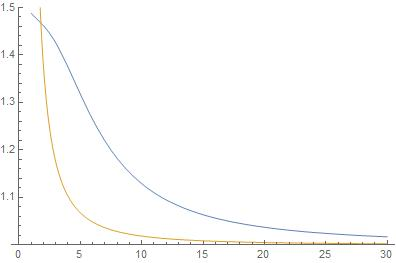
\includegraphics[width = 2\textwidth/3]{images/xCoefsTwoks.jpg}
    \caption{Matrix element $\langle \psi_{\Lambda} |\chi^+ | \psi_{\Lambda-1}\rangle = \langle \psi_{-\Lambda} |\chi^- | \psi_{1-\Lambda}\rangle$ as a function of $\Lambda$. Blue: for $k(\Lambda) = \frac{(\Lambda^2 + 18)^2}{18}$. Yellow: for $k(\Lambda) = \Lambda^2(\Lambda+1)^2$.}
    \label{fig:originalbn}
\end{figure}

\begin{definition}\label{definitionChiPMChiiD2}
\emph{The normalization constant of the position operators} is the function in $k$:
\begin{eqnsplit}
    a(k) &:= %\sqrt{2}\langle \psi_1 | x^+ | \psi_0 \rangle = \sqrt{2}\langle \psi_{-1} | x^- | \psi_0 \rangle\\
    \langle \psi_1 | x^+ | \psi_0 \rangle = \langle \psi_{-1} | x^- | \psi_0 \rangle\\
    &= K_{0,1}(k) e^{\rho_{0,1}(k) + \frac{1}{4c_{0,1}(k)}}\\
    &= 1 + \frac{9}{4\sqrt{2}} \frac{1}{\sqrt{k}} + \frac{137}{64} \frac{1}{k} + \frac{715}{256 \sqrt{2}} \frac{1}{k^{\frac{3}{2}}} + O(\frac{1}{k^2})
\end{eqnsplit}
\emph{The normalized position operators} are, for $i = 1, 2$:
\begin{eqnsplit}
    \chi^i &:= \frac{\cut{x^i}}{a(k)}\\
    \chi^\pm &:= \frac{\cut{x^\pm}}{a(k)} = \chi^+ \pm i \chi^-.
\end{eqnsplit}%\todo{In the last papers the $\pm$ ones include a factor of $\sqrt{2}$ in front, but I don't think it is important}
\end{definition}

The normalization constant $a$ is simply the factor that extracts the $m$ independent terms in the series expansion of the action of $\cut{x^\pm}$ on each $\psi_m$. $a$ rapidly converges to $1$ with increasing $k$, as shown in the figure \ref{fig:asolo}.% graph \ref{fig:acomparados} shows the some approximate values of $a$ plotted besides the theoretical value of $a$.
\begin{figure}[h]
    \centering
    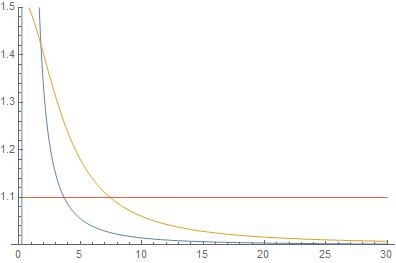
\includegraphics[width = 2\textwidth/3]{images/asolo.jpg}
    \caption{Normalizing factor $a$ as a function of $\Lambda$. Yellow: for $k(\Lambda) = \frac{(\Lambda^2 + 18)^2}{18}$. Blue: for $k(\Lambda) = \Lambda^2(\Lambda+1)^2$.}
    \label{fig:asolo}
\end{figure}

\begin{proposition}%\todo{the notation for $m$ is bad, but it is for me to remember that perhaps something should be said about how the powers of $m$ increase with the powers of $k$}
Up to second order of powers in $\frac{1}{\sqrt{k}}$ in the coefficients the following relations hold:
\begin{align}\label{equationActionChiD2WithoutOO}
    \chi^\pm  \psi_m
        &= \begin{cases}
        %\frac{1}{\sqrt{2}}\sqrt{1 + \frac{m(m+1)}{k}}  \psi_{m \pm 1} & \text{if } -\Lambda \leq \pm m \leq \Lambda -1
        \sqrt{1 + \frac{m(m+1)}{k}}  \psi_{m \pm 1} & \text{if } -\Lambda \leq \pm m \leq \Lambda -1
        \\
        0 & \text{otherwise}
        \end{cases}\\
    \label{equationCommutatorChiD2}
    [\chi^+, \chi^-]  \psi_m
        &= \begin{cases}
         -\frac{2m}{k} \psi_{m} & \text{if } |m| \leq \Lambda -1
        \\
        \pm \left( 1 + \frac{\Lambda(\Lambda-1)}{k} \right) \psi_{m} & \text{if } m = \pm \Lambda 
        \end{cases}\\
    \label{equationRChiD2}
    \vec \chi^2  \psi_m
        &= \begin{cases}
        \left( 1+ \frac{m^2}{k} \right) \psi_{m} & \text{if } |m| \leq \Lambda -1
        \\
        \frac{1}{2} \left( 1+ \frac{\Lambda(\Lambda-1)}{k} \right) \psi_{m} & \text{if } m = \pm \Lambda 
        \end{cases}
\end{align}
where $\vec \chi^2 := (\chi^1)^2 + (\chi^2)^2 = \frac{1}{2}(\chi^+\chi^- + \chi^-\chi^+)= R^2/a^2$.
\end{proposition}
The coefficient $\langle \psi_{m \pm 1} \chi^+ | \psi_{m}\rangle$ is visualized in figures \ref{fig:figureabnChiMinK} and \ref{fig:figureabnChiRecommendedK}.

\begin{figure}[h]
    \centering
    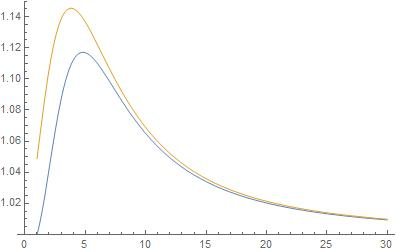
\includegraphics[width = 2\textwidth/3]{images/divFactorwMinimumK.jpg}
    \caption{Maximum value of coefficient $\langle \psi_{m \pm 1} |\chi^\pm | \psi_{m}\rangle$ as a function of $\Lambda$ for $k(\Lambda) = \frac{(\Lambda^2 + 18)^2}{18}$. Blue: exact value. Yellow: approximation $\sqrt{1 + \frac{\Lambda(\Lambda+1)}{k}}$.}
    \label{fig:figureabnChiMinK}
\end{figure}

\begin{figure}[h]
    \centering
    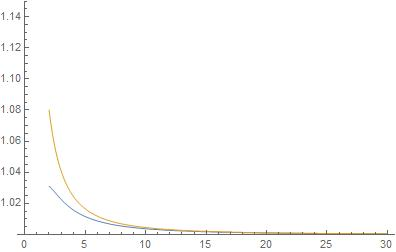
\includegraphics[width = 2\textwidth/3]{images/divFactorwRecommendedK.jpg}
    \caption{Maximum value of coefficient $\langle \psi_{m \pm 1} |\chi^\pm | \psi_{m}\rangle$ as a function of $\Lambda$ for $k(\Lambda) = \Lambda^2(\Lambda+1)^2$. Blue: exact value. Yellow: approximation $\sqrt{1 + \frac{\Lambda(\Lambda+1)}{k}}$.}
    \label{fig:figureabnChiRecommendedK}
\end{figure}

\begin{remark}
Notice that if the action \eqref{equationActionChiD2WithoutOO} were used exactly to define operators $\chi^\pm$, then equations \eqref{equationCommutatorChiD2} and \eqref{equationRChiD2} would also be exact. This is thanks to the fact that, although the square root in \eqref{equationActionChiD2WithoutOO} is only valid up to the power $\frac{1}{k}$, i.e. it is only meaningful to say that it is equal to $ 1+\frac{m(m+1)}{2}$, when we use it to calculate the commutator and the radius it produces precisely the correct first order terms stated above.
\end{remark}

\begin{theorem}[Summary]
$\chi^+$ and $\chi^-$ generate the $*$-algebra $\acal_\Lambda = End(\hcal_\Lambda)$. The generators $\chi^\pm$ and $\cut L$ satisfy \todo{does this characterize algebraically the algebra?} the relations:
\begin{align}\label{equationOperatorFormulaRelationsChiD2}
    (\chi^+)^{2\Lambda+1} &= 0, & 
    (\chi^-)^{2\Lambda+1} &= 0, & 
    (\chi^+)^*&= \chi^-, & 
    \prod_{m = \Lambda}^\Lambda (\cut L - m), &= 0 & 
    \cut L^* &= \cut L,
\end{align}
\begin{align}\label{equationOperatorFormulaCommutatorsChiD2}
    [\cut L, \chi^\pm] &= \pm \chi^\pm,&
    [\chi^+, \chi^-] &= - \frac{2\cut L}{k} + \left[ 1 + \frac{\Lambda(\Lambda+1)}{k}\right](\tilde P_\Lambda - \tilde P_\Lambda),
\end{align}
where the projections $\tilde P_m$ are polynomials in $\cut L$. Furthermore,
\begin{equation}\label{equationOperatorFormulaRChiD2}
    \vec \chi^2 = 1 + \frac{L^2}{k} - \left[ 1 + \frac{\Lambda(\Lambda+1)}{k}\right]\frac{\tilde P_\Lambda - \tilde P_\Lambda}{2}.
\end{equation}
Equations \eqref{equationOperatorFormulaCommutatorsChiD2}$_2$ and \eqref{equationOperatorFormulaRChiD2} are only valid up to second order in powers of $\frac{1}{\sqrt{k}}$; however, if the formulas \eqref{equationActionChiD2WithoutOO} are used as exact definitions of $\chi^\pm$, then all the equations in this theorem are satisfied exactly.
\end{theorem}


% {\color{gray}
% In some sense $\cut L \to L$. In what sense?\todo{} What about the $x^\pm$ and the $\xi^\pm$?\todo{}

% $\cut{\partial_{\pm}}$ are not needed as generators, and they do not go to $\partial_\pm$ since they can't replicate the emergence of an $n = 1$ component when acting on $\psi_m$ by $\partial_\pm$.
% }





%%%%%%%%%%%%%%%%%%%%%%%%%%%%%%%%%%%%%%%%%%%%%%%%%%%%%%%%%%%%%%%%
%%%%%%%%%%%%%%%%%%%%%%%%%%%%%%%%%%%%%%%%%%%%%%%%%%%%%%%%%%%%%%%%
\section{Realization of $\acal_\Lambda$ through $U(\soth)$}

% {
%     % \color{gray}
    
%     % - $O(2)$ acts on $\hcal_\Lambda \subset L^2(\RR^2)$, and so \rtext{on $\acal_\Lambda$}, since $[H, O(2)\cdot ] = 0$. through the action induced in $\acal_\Lambda$ by its action on $\RR^2$. Furthermore, its action is the one expected on position coordinates:
%     %     \begin{itemize}
            
%     %     \item \emph{Rotation} $R_\theta$: $\cut{x^\pm} \mapsto e^{\pm i \theta} \cut{x ^\pm}; \cut L \mapsto \cut L \in \acal_\Lambda$.
        
%     %     \item \emph{Reflection}: $\cut{x^\pm} \mapsto -\cut{x^\mp}; \cut L \mapsto -\cut L$.
        
%     %     \end{itemize}
    
%     % - \rtext{We can consider \otext{$\acal_\Lambda \cong  M_N(\CC) = \pi_\Lambda(Uso(3))$} \textbf{as a $*$-algebra and representations of $O(2)$}}, where $\pi_\Lambda$ is the $\lbtext{N} := 2 \Lambda + 1$ dimensional representation. $SU(N) \ni g$ is the group of $*$-automorphisms of $M_N(\CC) \cong \acal_\Lambda$ acting by $a \mapsto g a g^{-1}$; $O(2)$ is then a subgroup. Comes from mapping:
%     % \begin{align}
%     %     \rtext{\cut{x^\pm}} &\longleftrightarrow \rtext{f_\pm (J^0) J^\pm}, &
%     %     \rtext{\cut L }& \rtext{\longleftrightarrow J^0}
%     % \end{align}
%     % where $J^\pm, J^0$ is the Weyl-Cartan basis of $so(3)$, $\lbtext{f_\pm(s)} := \frac{1}{\sqrt{2}} \sqrt{\frac{1 + s(s-1)/k}{\Lambda (\Lambda + 1) - s(s-1)}} =: \lbtext{f_-(-s)}$%: $[J^+, J^-] = J^0; [J^\pm, J^0] = \pm J^\pm$

%     % - $O(2) \subset SO(3)$: \emph{Rotation}: $\pi_\Lambda(e^{i \theta J_0})$; \emph{Refl.}: $\pi_\Lambda(e^{i\pi (J^+ + J^-)/\sqrt{2}})$
    
%     \lin 
    
%     Let $(V_l, \pi_l)$ be the irreducible representations of $O(2)$ characterized by $L^2 = l^2$
    
%         \begin{itemize}
        
%         \item  \begin{equation}
%             \hcal_\Lambda \cong \bigoplus_{l = 0}^\Lambda V_l
%         \end{equation}
        
%         \item \begin{equation}
%             C_\Lambda \cong \bigoplus_{l = 0}^{2\Lambda} V_l
%         \end{equation}
        
%         \end{itemize}
        
%     \rtext{\textbf{As $\Lambda \to \infty$ these respectively become the decomposition of $L^2(S^2)$ \& of $C(S^2)$ that acts on $L^2(S^2)$.}}
% }



Throughout this section let $\Lambda \in \NN$ and let $\acal_\Lambda$ and $\hcal_\Lambda$ be defined as in Definition \ref{definitionHLambdaALambdaD2}.

\begin{lemma}\label{lemmaExistsPolynomialInLTakingSameGradeToItD2}
Let $A_1, A_2$ be elements of $\acal_\Lambda^n$, and suppose that $A_1 \psi_m = 0$ implies that $A_2\psi_m = 0$ for $m \in \{-\Lambda, \dots, \Lambda\}$.
Then there is a polynomial $f(\cut L)$ in $\cut L$ such that $A_2 = f(\cut L) A_1$. Furthermore, if $f'$ is another polynomial such that $f'(\cut L)\psi_m = f(\cut L)\psi_m$ whenever $A_1 \psi_m \neq 0$, then it is also satisfied that $A_2 = f'(\cut L) A_1$.
\end{lemma}
\begin{proof}
Let $g_1, g_2$ be functions on $m \in \{-\Lambda, \dots, \Lambda\}\subset \ZZ$ such that $A_i = \sum_{m: \, |m+n| \leq \Lambda} g_i(m) S^{n-m} \tilde P_m$, where $S^{\pm 1}$ are ladder operators; notice that $g_i(m)$ is arbitrary when $A_i \psi_m = 0$, in particular on $m$ such that $|m+n| > \Lambda$, so we may choose the $g_i$ nowhere $0$. Define $f(m) = \frac{g_2(m-n)}{g_1(m-n)}$ if $|m+n| \leq \Lambda$, and choose it arbitrarily for the the remaining $m \in \{-\Lambda, \dots, \Lambda\}$. Thus, any polynomial $f(\cut L) := \sum_{m} f(m) \tilde P_m$ defined with such a function $f$ on $\{-\Lambda, \dots, \Lambda\}$ makes the equation $A_2 = f(\cut L) A_1$ be satisfied.
\end{proof}

\begin{proposition}\label{propositionThereAreFunctionsfpmD2}
Let $L^\pm \in \acal_{\Lambda}$ be defined by
\begin{align}
    L^\pm \psi_m &:= \sqrt{\Lambda(\Lambda + 1) - m(m \pm 1)}& \text{for all }m \in \{-\Lambda, \dots, \Lambda\}\subset \ZZ.
\end{align}
Then, $L^\pm$ generate $\acal_\Lambda$ and there are polynomials $f^x_\pm(L)$, $f^\chi_\pm$, $f_\pm$ in $\cut L$ such that
\begin{align}
    \cut{x^\pm} &= f^x_{\pm}(\cut L) L^\pm,&
    \cut{\chi^\pm} &= f^\chi_{\pm}(\cut L) L^\pm;
\end{align}
any such polynomials have the property that, for $|m \pm 1| \leq \Lambda$, the functions
\begin{align}\label{equationApproximatedfPolynomialLForVanillaX}
    f^x_\pm(m) &:= f^x_\pm(L)\psi_m = \frac{1 + \frac{9\sqrt{2}}{8}\frac{1}{\sqrt{k}} + \frac{137 \pm 32(m \mp 1) + 32(m \mp 1)^2}{64}\frac{1}{k}}{\sqrt{\Lambda(\Lambda+1) - m(m \mp 1)}}\\
    \label{equationApproximatedfPolynomialLForChiWithoutOOs}
    f^\chi_\pm(m)&:= f^\chi_\pm(L)\psi_m = \sqrt{\frac{1 + \frac{m(m\mp 1)}{k}}{\Lambda(\Lambda+1) - m(m \mp 1)}}
\end{align}
satisfy the equalities above up to second order in powers of $\frac{1}{\sqrt{k}}$. 

Similarly, if equations \eqref{equationActionChiD2WithoutOO} are used exactly to define the operators $\chi^\pm \in \acal_\Lambda$, then equation \eqref{equationApproximatedfPolynomialLForChiWithoutOOs} is exact too.
\end{proposition}
\begin{proof}
That $L^\pm$ are generators of $\acal_\Lambda$ is a direct combination of lemmas \ref{lemmaLUDScalarAngularMomentumGenerateD2} and \ref{lemmaLIsPolynomialOfUpDownLaddersD2}.

The rest of the statement is a corollary of Lemma \ref{lemmaExistsPolynomialInLTakingSameGradeToItD2}, where the polynomial $f^x_\pm(\cut L)  \equiv \sum_m f^x(m) \tilde P_m$ in $\cut L$ are defined by the fact, $\cut{x^\pm} \psi_m = f^x_\pm(m) L^\pm \psi_m$ on those $m$ such that $|m \pm 1| \leq \Lambda$; there is no restriction on what $f^x_\pm(\pm \Lambda)$ should be, since the evaluation of the polynomial isn't ever done on $\psi^{\pm \Lambda}$. The same reasoning applies to $f^\chi_\pm$.
\end{proof}

\lin 

As we saw in Chapter \ref{chp:fuzzysphere}, an important component of a fuzzy space is its action under a symmetry group. It was remarked \ref{remarkODActsOnHCutE} that the left action of $O(2) \ni g$ on $\RR^2$ induced a unitary representation $\hat \pi: O(2) \to \bcal(L^2(\RR^2))$, which in turn induces a left action of $O(2)$ on $\acal_{\cut E} \ni A$ by inner isomorphisms $A^g = \pi'(g) A \pi'(g)^*$, for any cutoff energy $\cut E \geq 0$ and compatible $k$. It was further proved in theorem \ref{theoremGeneralDEffectiveLowEnergyQuantumIsODCovariant} that the operators $\cut {x^i}$, $i = 1, 2$, transform contravariantly under $O(2)$. We will now see how this action looks for of the operators that we have used so far for the algebras $\acal_\Lambda$ for arbitrary $\Lambda \in \NN$, where we will call by $\hat \pi_\Lambda$ the representation of $O(2)$ on $\hcal_\Lambda$.%, as well as the induced algebra representation of $U()$

First, recall that the group of rotations on $\RR^2$ is precisely the subgroup $SO(2) \subset O(2)$ of elements of determinant $1$, instead of $-1$. Furthermore, every rotation is determined by the angle $\theta \in [0, 2\pi]$ that the $x^1$-axis rotates in the anticlockwise direction; hence, every rotation is of the form
\begin{equation}\label{equationGEneral2DRotationTheta}
    R_\theta := 
    \begin{pmatrix}
    \cos \theta & -\sin \theta \\
    \sin \theta & \cos \theta
    \end{pmatrix}.
\end{equation}
Additionally, let
\begin{equation}
    F := \begin{pmatrix}
    1 & 0 \\
    0 & -1
    \end{pmatrix}
\end{equation} be the element of $O(2)$ of determinant $-1$ that represents the reflection with respect to the $x^1$-axis. Then, every element $g \in O(2)$ whose determinant isn't $1$, i.e. it is $-1$ is such that $Fg \in SO(2)$, and so every element of determinant $-1$ in $O(2)$ can be written as the product of a rotation with $F$; this all combines to the fact that the group $O(2)$ is generated by the space of rotations together with the reflection $F$.

The contravariant transformation $\pi(g)'\cut{x^i} \pi(g)^* = \sum_j (g^T)^i_j \cut{x^j}$ of the operators $\cut{x^i}$ under the rotation $g = R_\theta$ looks as follows:
\begin{eqnsplit}
    (\cut{x^1})^{R_\theta} &= \pi(R_\theta)'\cut{x^i} \pi(R_\theta)*\\ &=\cut{x^1} \cos \theta + \cut{x^2} \sin \theta,\\
    (\cut{x^2})^{R_\theta} &= -\cut{x^1} \sin \theta + \cut{x^2} \cos \theta.
\end{eqnsplit}
Similarly, the (contravariant) transformation under the reflection $F$ is
\begin{eqnsplit}
    (\cut{x^1})^{F} &= \cut{x^1},\\
    (\cut{x^2})^{F} &= -\cut{x^2}.
\end{eqnsplit}
This all implies that the action on the operators $\cut{x^\pm} = \cut{x^1} + i \cut{x^2}$ is
\begin{eqnsplit}\label{equationActionO2xpmD2}
    (\cut{x^\pm})^{R_\theta} &= e^{-i \theta} x^\pm,\\
     (\cut{x^\pm})^F &= x^{\mp};
\end{eqnsplit}
we will call this transformation rule for operators $U \in \acal_\Lambda^1$ and $D \in \acal_\Lambda^{-1}$ \emph{a contravariant transformation of the operators $U, D$}.

Now, on $\RR^2$, $\pi(R_\theta)\partial_\phi \pi(R_\theta)*\psi(r, \phi) = \pi(R_\theta)\partial_\phi \psi(r, \phi+ \theta) = \pi(R_\theta) \partial_\phi \psi(r, \phi + \theta) = \pi(R_\theta) \partial_{\phi+\theta} \psi(r, \phi + \theta) = \partial_\phi \psi(r, \phi)$ for all $\psi \in L^2(\RR^2)$ i.e. $(\partial_\phi)^{R_\theta} = \partial_\phi$, then we have that $L^{R_\theta} = L$ and so, since $[P_\Lambda, \pi'(R_\theta)] = 0$, that
\begin{equation}
    (\cut L)^{R_\theta} = \cut L.
\end{equation}
Similarly, since $\phi = \arctan{\frac{x^2}{x^1}}$ in $\RR^2$, the action by the reflection $F \in O(2)$ on $\cut L$ is
\begin{equation}
    (\cut L)^F = - \cut L.
\end{equation}

Now, notice that since $\chi^i = \frac{\cut{x^i}}{a(k)}$, then $\chi^\pm$ has the same transformation laws under $O(2)$ as $\cut{x^\pm}$, hence
\begin{eqnsplit}\label{equationActionO2ChipmD2}
    (\chi^\pm)^{R_\theta} &= e^{\mp i\theta} \chi^\pm;\\
    (\chi^\pm)^F &= \chi^\mp.
\end{eqnsplit}

Similarly, the operators $L^\pm$ defined in proposition \ref{propositionThereAreFunctionsfpmD2} also have a contravariant transformation law under $O(2)$. To see this, first notice that we may write $L^\pm =  (f^\chi_\pm)^{-1}(\cut L) x^\pm$, where $(f^\chi_\pm)^{-1}(\cut L)$ is the polynomial such that $(f^\chi_\pm)^{-1}(m) := (f^\chi_\pm)^{-1}(\cut L)\psi_m = \frac{1}{f^\chi_\pm(m)}$. Also notice that $\pi'(g) (f^\chi_\pm)^{-1}(\cut L) \pi'(g)^* = (f^\chi_\pm)^{-1}(\pi'(g)\cut L \pi'(g)^*)$ for all $g \in O(2)$, so $\pi'(R_\theta) (f^\chi_\pm)^{-1}(\cut L) \pi'(R_\theta)^* = (f^\chi_\pm)^{-1}(\cut L)$ and 
$\pi'(F) (f^\chi_\pm)^{-1}(\cut L) \pi'(F)^* = (f^\chi_\pm)^{-1}(-\cut L) = (f^\chi_\mp)^{-1}(\cut L)$, where the last equation follows from the fact that, as polynomials in $\cut L$, $\tilde P_m(-\cut L) = \tilde P_{\cut L}(\cut L)$ and from the equation $f^\chi_\pm(-m) = f^\chi_\mp(m)$. Thus,
\begin{eqnsplit}\label{equationTransformationLawLpmD21}
    \pi'(R_\theta) L^\pm \pi'(R_\theta)^* &= \pi(R_\theta)(f^\chi_\pm)^{-1}(\cut L)\pi(R_\theta)^* \pi'(R_\theta) \chi^\pm \pi'(R_\theta)^*\\
    &= (f^\chi_\pm)^{-1}(\cut L) e^{\mp i \theta} \chi^\pm\\
    &= e^{\mp i \theta} L^\pm,
\end{eqnsplit} and
\begin{eqnsplit}\label{equationTransformationLawLpmD22}
    \pi'(F) L^\pm \pi'(F)^* &=  \pi'(F)(f^\chi_\pm)^{-1}(\cut L)\pi'(F)^* \pi'(F) \chi^\pm \pi'(F)^*\\
    &= (f^\chi_\mp)^{-1}(\cut L) \chi^\mp\\
    &= L^\mp.
\end{eqnsplit}


\lin

We will now see that the algebras $\acal_{\Lambda}$ developed in this chapter can be more concisely understood as the algebras of endomorphisms of irreducible representation spaces of $SO(3)$, just like the even-indexed elements of the fuzzy sphere. Recall that $\hat \pi_\Lambda$ denotes the representation of both $SO(3)$ on the representation spaces of $SU(2)$ $V_{\Lambda} \cong \CC^{2\Lambda + 1}$, which is induced by the representation $\pi_\Lambda$ of $SU(2)$. Let us also denote by $\hat \pi$ the algebra representation of $U(\soth)$ induced by the group representation $\hat \pi$, and recall that $i\hat J^k \in U(\soth)$, $k = 1, 2, 3$, is the infinitesimal rotation in $\RR^3$ about the $i$-th axis.

Since $V_\Lambda$ is a representation space of $SO(3)$, by identifying $O(2)$ as a subgroup of $SO(3)$ we can then restrict $\hat \pi$ to $O(2)$ to get a representation of it on $V_\Lambda$, and therefore a left action of $O(2)$ on $\acal_\Lambda$. Let us make the following identifications
\begin{align*}
    O(2) && \hookrightarrow && SO(3)\\
    R_\theta && \mapsto && \begin{pmatrix} R_\theta & 0 \\ 0 & 1 \end{pmatrix} = e^{i\theta \hat J^3}\\
    F && \mapsto && e^{i\pi \hat J^1};
\end{align*}
we can see that the subgroup of $SO(3)$ generated by the elements of the form $e^{i\theta \hat J^3}$ and $e^{i\pi \hat J^3}$ is isomorphic to $O(2)$, by realizing that it acts on the plane $x^1-x^2$ in $\RR^3$ precisely as $O(2)$ acts on $\RR^2$.

\begin{theorem}\label{theoremUso3ViewAlternativeAlgebraO2IsomorphismD2}
For all $\Lambda \in \NN$, let $T: \hcal_\Lambda \to V_\Lambda$ be the isomorphism of the Hilbert spaces $\hcal_\Lambda \subset L^2(\RR^2)$ and $V_\Lambda \equiv \CC^{2\Lambda + 1}$ generated by the mapping $\psi_m \mapsto |\Lambda, m\rangle$, $m \in \{-\Lambda, \dots, \Lambda\}$. Then, $T$ induces an isomorphism $\tilde T$ of the $C^*$-algebra $\acal_\Lambda = End(\hcal_)$, with the operator norm, is a $C^*$-algebra isomorphic to $\hat \pi_\Lambda(U(\soth)) = End(V_\Lambda)$ with the operator norm, and this isomorphism is $O(2)$-equivariant. Furthermore, the tuples of operators $(\tilde T(\cut{x^1}), \tilde T(\cut{x^2}))$ and $(\tilde T(\chi^1), \tilde T(\chi^2))$ transform $O(2)$-contravariantly.
\end{theorem}
\begin{proof}
First notice that $T: \hcal_\Lambda \to V_\Lambda$ is an isomorphism of Hilbert spaces since $\{\psi_m\}_{|m| \leq \Lambda} \subset \hcal_\Lambda$ and $\{|\Lambda, m\rangle\}_{|m| \leq \Lambda}$ are orthonormal basis of their respective space. The invertible mapping $\tilde T: \acal_\Lambda \to End(V_\Lambda)$ is defined as $A \mapsto T \circ A \circ T^{-1}$, and it clearly respects the algebra operations, i.e. it is an algebra isomorphism. This mapping is such that $\langle 
\psi_m | A | \psi^n \rangle = \langle \Lambda, m | \tilde T(A) | \Lambda, n\rangle$, for all $n, m \in \{-\Lambda, \dots, \Lambda\}$, and so $\tilde T$ respects adjoints, i.e. it is a $*$-isomorphism. Since $V_\Lambda \neq \{0\}$, for any $A \in \acal_\Lambda$:
\begin{align*}
    ||\tilde T (A)|| &= \sup_{v \in V_\Lambda} \{||\tilde T(A)(v)||\,:\, ||v|| = 1\} \\
    &= \sup_{\psi \in \hcal_\Lambda} \{||\tilde T(A)(T(\psi))||\,:\, ||T(\psi)|| = 1\} \\
    &= \sup_{\psi \in \hcal_\Lambda} \{||T(A(\psi))||\,:\, ||\psi|| = 1\} \\
    &= \sup_{\psi \in \hcal_\Lambda} \{||A(\psi)||\,:\, ||\psi|| = 1\}\\
    &= ||A||;
\end{align*}
hence $\tilde T$ respects the norm, so it is a Banach algebra isomorphism; notice that this boils down to the fact that $T$ is a normed vector space isomorphism, which itself is a consequence of the fact that $T$ maps an orthonormal basis to an orthonormal basis.

We now prove the $O(2)$-equivariance of $\tilde T$. Notice that 
\begin{equation}
    \tilde T(L^\pm) = \hat J^\pm,
\end{equation}
where $\hat J^\pm = \hat J^1 \pm i \hat J^2$, and $L^\pm$ are the algebra generators defined in proposition \ref{propositionThereAreFunctionsfpmD2}; this follows from the equation 
\[\langle \Lambda, n| \hat J^\pm |\Lambda, m \rangle = \delta_{n, m \pm 1} \sqrt{\Lambda(\Lambda + 1) - m(m \pm 1)} = \langle \psi_n | L^\pm | \psi_m \rangle,\]
for all $n, m \in \{-\Lambda, \dots, \Lambda\}$. Define the operators $L^1 = \frac{1}{2}(L^+ + L^-)$ and $L^2 = \frac{1}{2i}(L^+ - L^-)$; they satisfy that $\tilde T(L^k) = \hat J^k$, for $k = 1, 2$, and since $L^\pm$ generates $\acal_\Lambda$, then $L^1, L^2$ also generate it. Finally, the transformation laws \eqref{equationTransformationLawLpmD21} and \eqref{equationTransformationLawLpmD22} of $L^\pm$ imply that the operators $L^1$, $L^2$ transform contravariantly under $O(2)$, and so do $\hat J^1$, $\hat J^2$ under $O(2) \subset SO(3)$ as stated in proposition \ref{propositionMadoreCoordinatesAreSO3ContravariantCovariant}, recalling that $O(2) \subset SO(3)$ leaves invariant the third coordinate. Since $L^1, L^2$ generate $\acal_\Lambda$, the action of $O(2)$ on $\acal_\Lambda$ is completely determined by its action on $L^1$ and $L^2$; hence, that the mapping $L^k \mapsto \hat J^k$ is $O(2)$-covariant implies that $\tilde T$ is $O(2)$-equivariant, as desired.

The last part of the theorem follows from the $O(2)$-equivariance of $\tilde T$, together with the $O(2)$-contravariant transformations of $\cut{x^1}, \cut{x^2}$, and of $\chi^1, \chi^2$.
\end{proof}

\lin

Another $O(2)$-equivariant manifestation of the algebras $\acal_\Lambda$ can be achieved through $L^2(S^1)$:
\begin{definition}
For $\Lambda \in \NN$, let $\tilde\hcal_\Lambda \subset L^2(S^1)$ be the Hilbert space generated by the orthonormal set $\{e^{im\phi}\}_{|m|\leq \Lambda}$ with the inherited inner product, and let $\tilde \acal_\Lambda := End(\tilde \hcal_\Lambda)$. By abuse of notation, denote by $L$ and $x^\pm$ the restriction to $\tilde \hcal_\Lambda$ of the operators $L$ and $x^\pm$ on $L^2(S^1)$.
\end{definition}

Since $S^1 \subset \RR^2$, $O(2)$ acts naturally on each $\tilde \hcal_\Lambda$. Explicitly, 
\begin{eqnsplit}\label{equationTransformationO2OfeimphiHarmonicsCircled1}
    R_\theta \cdot e^{im\phi} &= e^{im(\phi - \theta)},\\
    F\cdot e^{im\phi} = e^{-im\phi},
\end{eqnsplit}
where $R_\theta$ is the anticlockwise rotation by $\theta \in [0, 2\pi]$ on $\RR^2$, and $\cdot$ denotes the (right) action of $O(2)$ on $\tilde \hcal_\Lambda$. Now, recall that $\psi_m \in \hcal_\Lambda$ has the form $\psi_m(\rho, \phi) = \tilde f(\rho) e^{im\phi}$, therefore
\begin{eqnsplit}\label{equationTransformationO2OfpsimhcalBasisD2}
    R_\theta \cdot \psi_m(\rho, \phi) &= \psi_m(\rho, \phi - \theta),\\
    F\cdot \psi_m(\rho, \phi) = \psi_m(\rho, -\phi),
\end{eqnsplit}
due to the fact that the radial coordinate is not affected by a $O(2)$ transformation, since, by definition, $O(2)$ doesn't change the metric in $\RR^2$. Thus, we can define the following alternative view of $\acal_\Lambda$:
\begin{theorem}\label{theoremEquivalent*IsomorphismALgebraSphericaleimphiD2}
For all $\Lambda \in \NN$, let $T: \hcal_\Lambda \to \tilde \hcal_\Lambda$ be defined by $\psi_m \mapsto e^{im\phi}$, for $m \in \{-\Lambda, \dots, \Lambda\}$. $T$ induces an isomorphism between the $C^*$-algebra $\acal_\Lambda$ is isomorphic to $\tilde \acal_\Lambda$ in an $O(2)$-equivariant way
\end{theorem}
\begin{proof}
The isomorphism $T: \hcal_\Lambda \to \tilde \hcal_\Lambda$ takes an orthonormal basis of $\hcal_\Lambda$ to an orthonormal basis of $\tilde \hcal_\Lambda$, hence, as seen in the proof of theorem \ref{theoremUso3ViewAlternativeAlgebraO2IsomorphismD2} this implies that the induced map on the algebras of endomorphisms in a $C^*$-algebra isomorphism.

The $O(2)$-equivariance follows from the equivalence of the transformation laws of the basis of these Hilbert spaces, stated in equations \eqref{equationTransformationO2OfeimphiHarmonicsCircled1} and \eqref{equationTransformationO2OfpsimhcalBasisD2}.

\end{proof}

%%%%%%%%%%%%%%%%%%%%%%%%%%%%%%%%%%%%%%%%%%%%%%%%%%%%%%%%%%%%%%%%
%%%%%%%%%%%%%%%%%%%%%%%%%%%%%%%%%%%%%%%%%%%%%%%%%%%%%%%%%%%%%%%%
\section{Convergence}

% {
%     \color{gray}
    
%     - \textbf{$\psi_m$ as fuzzy analogues of $e^{i m \phi} \in \hcal$}: $O(2)$-covariant embedding $\hcal_\Lambda \hookrightarrow \otext{\hcal = L^2(S^1)}$, $\psi_m \mapsto e^{im\phi}$; \hfill \\then $\hcal_\Lambda \to \hcal$ as $\Lambda \to \infty$ in the sense that $\forall \phi \in \hcal$, $\lbtext{\phi_\Lambda} := \sum_{|m| \leq \Lambda} \phi_m e^{im\phi} \to \phi$ in the $L^2$-norm.
    
%     - Induces, \rtext{embedding $\acal_\Lambda \hookrightarrow \otext{\acal = \mathcal B(\hcal)}$ and limit $\acal_\Lambda \to \acal$} as $\Lambda \to \infty$.
    
%     - \textbf{Fuzzy analogue of $B(S^1)$ of (bounded) functions on $S^1$} as subalgebra (act by mult.) of $\mathcal B(\hcal)$: $\lbtext{C_\Lambda} := \left\{ \sum_{h = -2\Lambda}^\Lambda f_h \eta^h \,|\, f_h \in \CC\right\}$ where $\eta^\pm  = \frac{\sqrt{2}}{a}x^\pm$ (so $\eta^\pm \to e^{\pm i \phi}$ as operators).
    
%     - Choosing $k(\Lambda) \geq 2 \Lambda(\Lambda + 1)(w\Lambda+1)^2$, then \rtext{$C_\Lambda \to C(S^1) \subset B(\hcal)$ as operators} due to the strong limits: $\hat f_\Lambda \to f\cdot$, $\hat{(fg)}_\Lambda \to fg\cdot $, $\hat f_\Lambda \hat g_\Lambda \to fg\cdot$, where $\lbtext{\hat f_\Lambda} := \sum_{h = -2\Lambda}^{2\Lambda} f_h \eta^h$ is ``truncation'' of $f \in B(S^1)$.
    
% }

% \linea

\subsection{To Quantum Mechanics on $S^1$}

In \cite{Fiore2018} the following type of convergence of a sequence of low energy effective theories with observable algebras $\{\acal_\Lambda\}_{\Lambda \in \NN}$ where each $\acal_\Lambda$ is as in Definition \ref{definitionHLambdaALambdaD2}:

Consider the $O(2)$-equivariant embedding $T: \hcal_\Lambda \to \tilde \hcal_\Lambda$ of theorem \ref{theoremEquivalent*IsomorphismALgebraSphericaleimphiD2}, as an identification of the two Hilbert spaces. We may say that we are considering the basis elements \emph{$\psi_m \in \hcal_\Lambda$ as the fuzzy analogs of $e^{im\phi}$}, when understood as elements of the Hilbert space $\hcal = L^2(S^1)$. For every $\varphi \in L^2(S^2)$, let $\varphi_\Lambda = \sum_{m = -\Lambda}^\Lambda \varphi_m e^{im\phi}$ where $\varphi_m$ are the Fourier coefficients of $\varphi$; $\varphi_\Lambda$ is identified via $T$ with $\sum_{m = -\Lambda}^\Lambda \varphi_m \psi_m$. Clearly $\phi_\Lambda \to \phi$ in the $L^2$-norm as $\Lambda \to 0$. In this sense Fiore and Pisacane in \cite{Fiore2018} then say that $\hcal_\Lambda$ \emph{invades} $\hcal$ as $\Lambda \to \infty$. 

Now, the identification $T$ induces an identification $\acal_\Lambda$ within $\bcal(L^2(S^1))$ as the algebra that annihilates $\tilde \hcal_\Lambda^\perp$ and whose application produces elements of $\tilde \hcal_\Lambda$. 

\begin{theorem}\label{theoremConvergesToQMD2}
Let $k(\Lambda)$ be any function satisfying inequality \eqref{inequationInequalityNeededforKasFunctionLambdaD2}. Under the identification $T: \hcal_\Lambda \to \tilde \hcal_\Lambda \subset \hcal$, then $\acal_\Lambda \subset \acal = \bcal (\hcal)$. Then the operators $\cut L $ converges strongly
\footnote{Ignoring domain issues, a sequence of operators $\{T_n\}_{n \in \NN}$ in a Banach space $V$ converges strongly to the operator $T$ with if, for all $v \in V$, $\lim_{n \to \infty} ||T_n v - T v|| \to 0$.}
 to $L$, and both $\chi^\pm$ and $\cut{x^\pm}$ converge strongly to $e^{\pm i\phi}$. If the operators $\chi^\pm$ are defined not as in Definition \ref{definitionChiPMChiiD2}, but via the exact action on the basis \eqref{equationActionChiD2WithoutOO}, the same convergence applies.

\noindent Since $L$ and $e^{\pm i \phi}$ generate the algebra of observables of a quantum particle in $S^1$, we then say that \emph{the limit of the low energy effective theories $\{(\hcal_\Lambda, \acal_\Lambda)\}$ is the quantum mechanics of a spin-less particle in $S^1$}.

\end{theorem}

\begin{proof}
Suppose that $\varphi$ is in the domain of $L$, i.e. $\sum_{m \in \ZZ} m^2 |\phi_m|^2 \leq \infty$, then
\begin{align*}
    ||(L - \cut L)\varphi|| = \sum_{|m| > \Lambda} m^2 |\phi_m|^2 \overset{\Lambda \to 0}{\longrightarrow} 0.
\end{align*}

Similarly, let $\varphi = \sum_{m \in \ZZ} \varphi_m e^{i \phi}$. Then
\begin{align*}
    ||(\chi^\pm - e^{\pm i \phi})\varphi||^2 &= \sum_{m = - \Lambda}^{\Lambda-1} \left[ \sqrt{1 + \frac{m(m \pm 1)}{k}} - 1 + O\left(\frac{m^3}{k^{\frac{3}{2}}} \right)\right] \varphi_m e^{i(m \pm 1)} - \sum_{m < \Lambda, m \geq \Lambda} \varphi_m e^{i(m \pm 1)}\\
    &\leq \sum_{m = -\Lambda}^{\Lambda-1} \left[\frac{m^2(m\pm 1)^2}{4k^2} + O\left(\frac{\Lambda^6}{k^{3}} \right)\right] |\varphi_m|^2 + \sum_{m < \Lambda, m \geq \Lambda} |\varphi_m|^2 \\
    &\leq \frac{\Lambda^2(\Lambda+1)^2}{4k^2} ||\varphi||^2 + \sum_{|m|\geq \Lambda} |\varphi_m|^2
\end{align*}
and this goes to $0$ when $\Lambda \to 0$ thanks to the inequality \eqref{inequationInequalityNeededforKasFunctionLambdaD2}; if the operators $\chi^\pm$ are defined by \eqref{equationActionChiD2WithoutOO}, the same calculation but removing the assymptotic terms applies. A similar argument follows for $\cut{x^\pm}$ since $\langle\psi_{m\pm 1} | \cut{x^\pm} | \psi_m\rangle - 1 = O\left(\frac{m}{k^{1/2}}\right) = O\left(\frac{\Lambda}{\Lambda^2} \right)$.
\end{proof}

Notice that $\chi^\pm$ nor $\cut{x^\pm}$ can converge in operator norm to $e^{\pm i\phi}$. Take for example $e^{i \lambda + 1} \in \hcal_\Lambda^\perp$, then $||(\chi^\pm -e^{\pm i m \phi})e^{i(\Lambda+1)\phi} || = ||0 - e^{i (\Lambda + 1 \pm 1) \phi}|| = 1$, meaning that $||\chi^\pm - e^{\pm i \phi}|| \geq 1$.

Notice that the transformation relations \eqref{equationTransformationO2OfpsimhcalBasisD2} imply that the spaces $W_{|m|} := span\{\psi_m, \psi_{-m}\}$, for $m \in \{-\Lambda, \dots, \Lambda\}$, are irreducible under the action of $O(2)$, and so
\begin{equation}
    \hcal_\Lambda = \bigoplus_{m = 0}^{\Lambda} W_m
\end{equation}
is the decomposition of $\hcal_\Lambda$ in irreducible representations of $O(2)$. Thus each $\hcal_\Lambda$ can be seen as the truncation of the decomposition
\begin{equation}
    L^2(S^1) = \bigoplus_{m  \in \NN} W_m.
\end{equation}

% As an $O(2)$-representation, $C_\Lambda$ has the decomposition
% \begin{equation}
%     C_\Lambda = \bigoplus_{m=0}^{2\Lambda} W_m,
% \end{equation}
% where $W_m = span\{\psi_m, \psi_{-m}\}$ for $m \in \{0, \dots, 2\Lambda\}$ given $\Lambda \in \NN$. This is a truncation of the decomposition
% \begin{equation}
%     \bcal(L^2(S^1)) = \bigoplus_{m=0}^{2\Lambda} W_m,
% \end{equation}

\subsection{To the Commutative Algebra $C(S^1)$}
%%%%%%%%%%%%%%%%%%%%%%%%%%%%%%%%%%%%%%%%%%%%%%%%%%%%%%%%%

Recall that in the canonical Dirac triple of a commutative space $X$, the commutative algebra $C(X)$ of continuous functions on $X$ has the role to act by multiplication on the Hilbert space of spinor fields. Since $S^1$ is a manifold or rank $1$, the fermionic Fock space has dimension $2^{\lfloor \frac{1}{2}\rfloor} = 1$, and the fact that $S^1$ is a compact simple Lie group means that its spinor bundle is a trivial\todo{DAndrea13 is the one who seems to say this} complex vector bundle\cite{}, hence it is simply $\hcal = L^2(S^1)$. Under some assumptions on the function $k(\Lambda)$, the identification of $\hcal_\Lambda$ with $\tilde \hcal_\Lambda$ through the $O(2)$-equivariant $*$-isomorphism $T$ of theorem \ref{theoremEquivalent*IsomorphismALgebraSphericaleimphiD2} will imply that the sequence of algebras $\{\acal_\Lambda\}_{\Lambda \in \NN}$ converge, in the sense soon to be specified, to the commutative subalgebra of $\bcal(\hcal)$ that the space $C(S^1)$ is.

In theorem \ref{theoremConvergesToQMD2} it was shown that $\chi^\pm$ and $\cut{x^\pm}$ converge strongly to the operator $e^{\pm i\phi}$, so let $x^\pm$ be either $\chi^\pm$ or $\cut{x^\pm}$; we might say that $x^\pm \in \acal_\Lambda$ are the fuzzy analogs of $e^{\pm i\phi}$, but as operators on $L^2(S^1)$. This suggests \cite{Fiore2018} the space (not an algebra)
\begin{equation}
    C_\Lambda := \left\{ \sum_{h = -2\Lambda}^{2\Lambda} f_h x^h \right\} \subset \acal_\lambda \subset \bcal(\hcal),
\end{equation}
where $x^h = (x^+)^h$ if $h \geq 0$ and $x^h = (x^-)^h$ if $h \leq 0$, as the fuzzy analog of $C(S^1)$, and in fact of the space of bounded functions $B(S^1)$, since they are the functions that have a Fourier series expansion that converges almost everywhere. For $f \in B(S^1)$, let $f = \sum_{h \in \ZZ} f_h e^{ih\phi}$ be its Fourier series, and define
\begin{equation}
    \hat f_\Lambda := \sum_{h = -2\Lambda}^{2\Lambda} f_h x^h;
\end{equation}
then it shown in \cite{Fiore2018} the following:

\begin{theorem}\label{theoremConvergesFuzzyCircleD2}
Suppose that $k(\Lambda) \geq 2\Lambda(\Lambda+1)(2\Lambda+1)^2$. Then, for all $f, g \in B(S^1)$ the following strong limits hold:
\begin{align}
    \hat f_\Lambda \to f\cdot && \hat{(fg)}_\Lambda \to fg\cdot && \hat f_\Lambda \hat g_\Lambda \to fg \cdot\,,
\end{align}
where the notation $f\cdot$ emphasizes $f$ as an operator on $\hcal$.
\end{theorem}

% %%%%%%%%%%%%%%%%%%%%%%%%%%%%%%%%%%%%%%%%%%%%%%%%%%%%%%%%%%%%%%%%
% %%%%%%%%%%%%%%%%%%%%%%%%%%%%%%%%%%%%%%%%%%%%%%%%%%%%%%%%%%%%%%%%
% \section{Conclusions and Outlook}

% % {\color{gray}

% %     By introducing a cutoff, we obtained a low energy effective of the quantum theory of a spin-less particle on $S^d$.
    
% %     We can use this construction to produce fuzzy spaces that approximate the classical configuration space $S^1$.
    
% %     If I do $D = 3$, I will be able to compare it with the traditional Fuzzy Sphere, and perhaps conclude (as they do) that this one is better.
% % }